% આ ભાગનો પૂર્ણ સંપાદનીય પાઠ છે. શૈલી, ફોન્ટ, ચિત્રો અને પ્રકરણસંદર્ભ માટે સંપૂર્ણ સ્રોત ZIP તથા reader/full-reader.tex જુઓ. આ એકલી સ્વતંત્ર કમ્પાઇલ થતી મુખ્ય ફાઇલ નથી.

% BEGIN OLP-0620
\olpart{his}{ઇતિહાસ}
\phantomsection\label{guunit:OLP-0620}


\begingroup
\makeatletter\def\ol@sectioncs{section}\makeatother

% BEGIN OLP-0621
\olchapter{his}{bio}{જીવનચરિત્રો}
\olchapterid{his}{bio}
\phantomsection\label{guunit:OLP-0621}


\begingroup
\makeatletter\def\ol@sectioncs{section}\makeatother

% BEGIN OLP-0622
\olfileid{his}{bio}{can}

\olsection{જ્યૉર્જ કૅન્ટૉર}
\phantomsection\label{guunit:OLP-0622}


\olphoto{cantor-georg}{જ્યૉર્જ કૅન્ટૉર}

જ્યૉર્જ કૅન્ટૉર (ઉચ્ચાર: ગે-ઓર્ગ કાન-ટોર)ના
એક પ્રારંભિક જીવનચરિત્રમાં
દાવો કરાયો હતો કે રશિયાના સેન્ટ પીટર્સબર્ગ તરફ
જતા જહાજમાં તેમનો જન્મ થયો, તેઓ ત્યાં મળી આવ્યા,
અને તેમના માતાપિતા કોણ હતા તે અજાણ્યું હતું.
પરંતુ આ સાચું નથી; તેમનો જન્મ 1845માં સેન્ટ
પીટર્સબર્ગમાં થયો હતો.

કૅન્ટૉરે 1867માં બર્લિન યુનિવર્સિટીમાંથી
ગણિતમાં ડૉક્ટરેટ મેળવી. ગણસિદ્ધાંતમાંના તેમના
કાર્ય માટે તેઓ જાણીતા છે, અને ગણસિદ્ધાંતને
અલગ સંશોધનક્ષેત્ર તરીકે સ્થાપવાનો શ્રેય તેમને
આપવામાં આવે છે. જુદા કદના અનંત ગણો હોય છે
તે સૌપ્રથમ તેમણે સાબિત કર્યું. તેમના સિદ્ધાંતો,
ખાસ કરીને અનંતતાઓનો સિદ્ધાંત, તે સમયના
ગણિતજ્ઞોમાં ઘણી ચર્ચાનું કારણ બન્યા અને તેમનું
કાર્ય વિવાદાસ્પદ રહ્યું.

કૅન્ટૉરની ધાર્મિક માન્યતાઓ અને તેમનું ગાણિતિક
કાર્ય અવિભાજ્ય રીતે જોડાયેલાં હતાં; તેમણે
એવો પણ દાવો કર્યો કે અનંતાતીત સંખ્યાઓનો
સિદ્ધાંત ઈશ્વરે તેમને સીધો જણાવ્યો હતો.
જીવનના પાછળના સમયગાળામાં કૅન્ટૉરને માનસિક
બીમારી થઈ. 1894થી અને પછીનાં વર્ષોમાં વધુ
વાર તેમને હોસ્પિટલમાં દાખલ કરાયા. તેમના
કાર્યની કઠોર ટીકા, જેમાં ગણિતજ્ઞ લિયોપોલ્ડ
ક્રોનેકર સાથેનો સંબંધવિચ્છેદ પણ હતો, તેમને
અવસાદ તરફ અને ગણિતમાં રસ ઘટવા તરફ દોરી ગઈ.
અવસાદના પ્રસંગોમાં કૅન્ટૉર તત્ત્વચિંતન અને
સાહિત્ય તરફ વળતા. તેમણે ફ્રાન્સિસ બેકન
શેક્સપિયરના નાટકોના લેખક હતા એવો સિદ્ધાંત
પણ પ્રકાશિત કર્યો.

કૅન્ટૉરનું અવસાન 6 જાન્યુઆરી 1918ના રોજ
હાલેના એક સેનેટોરિયમમાં થયું.

\begin{reading}
કૅન્ટૉરનાં વિગતવાર જીવનચરિત્રો માટે
\citet{Dauben1990} અને
\citet{Grattan-Guinness1971} જુઓ. તેમના
ક્રાંતિકારી વિચારોનું વર્ણન બીબીસી રેડિયો 4ના
\emph{A Brief History of
  Mathematics} કાર્યક્રમમાં પણ છે
\citep{Sautoy2014}. કૅન્ટૉરના સિદ્ધાંતો
રેપ સ્વરૂપે સાંભળવા હોય તો \citet{Rose2012} જુઓ.
\end{reading}
% END OLP-0622
\endgroup


\begingroup
\makeatletter\def\ol@sectioncs{section}\makeatother

% BEGIN OLP-0623
\olfileid{his}{bio}{chu}

\olsection{અલોન્ઝો ચર્ચ}
\phantomsection\label{guunit:OLP-0623}


\olphoto{church-alonzo}{અલોન્ઝો ચર્ચ}

અલોન્ઝો ચર્ચનો જન્મ 14 જૂન 1903ના રોજ
વૉશિંગ્ટન, ડી.સી.માં થયો હતો. નાનપણમાં
હવાઈ બંદૂક સાથેની ઘટનાને કારણે તેમની
એક આંખની દૃષ્ટિ જતી રહી. તેમણે 1920માં
કનેક્ટિકટમાં યુનિવર્સિટી-પૂર્વ શાળાનો અભ્યાસ પૂરો
કર્યો અને એ જ વર્ષે પ્રિન્સ્ટનમાં
યુનિવર્સિટીનો અભ્યાસ શરૂ કર્યો. 1927માં
તેમણે ડૉક્ટરેટનો અભ્યાસ પૂરો કર્યો.
કેટલાંક વર્ષ વિદેશમાં વિતાવ્યા પછી ચર્ચ
પ્રિન્સ્ટન પરત ફર્યા. તેઓ અત્યંત વિનમ્ર
અને ચીવટવાળા તરીકે જાણીતા હતા. બોર્ડ
પરનું તેમનું લખાણ એકદમ સ્વચ્છ હોતું,
અને મહત્વના કાગળોને સાચવવા તેઓ તેને
પારદર્શક ગુંદર, ડ્યુકો સિમેન્ટ, વડે
કાળજીપૂર્વક ઢાંકતા. શૈક્ષણિક કાર્ય
સિવાય તેમને વિજ્ઞાનકથાની સામયિકો
વાંચવાનો શોખ હતો; લેખનમાં ભૂલ દેખાય
તો સંપાદકોને લખતાં પણ તેઓ અચકાતા નહીં.

ચર્ચની શૈક્ષણિક સિદ્ધિઓ મોટી હતી.
તેમના વિદ્યાર્થીઓ સ્ટીફન ક્લીની અને
બાર્કલી રોસેર સાથે તેમણે અસરકારક
સંગણનીયતાનો સિદ્ધાંત, લૅમ્બડા કલન,
વિકસાવ્યો; એલન ટ્યુરિંગે ટ્યુરિંગ
મશીન વિકસાવ્યું તેનાથી આ કાર્ય સ્વતંત્ર
હતું. સંગણનીયતાની આ બે વ્યાખ્યાઓ
સમકક્ષ છે અને આજે જેને
\emph{ચર્ચ--ટ્યુરિંગ માન્યતા} કહે છે
તે તરફ દોરી જાય છે: પ્રાકૃતિક સંખ્યાઓ
પરનું વિધેય અસરકારક રીતે સંગણનીય હોય
ત્યારે અને ત્યારે જ જ્યારે તેને
ટ્યુરિંગ મશીન (અથવા લૅમ્બડા કલન)
વડે ગણી શકાય. તેમણે આજે
\emph{ચર્ચનું પ્રમેય} કહેવાતું પરિણામ
પણ સાબિત કર્યું: પ્રથમ-ક્રમનાં સૂત્રોનું
પ્રામાણ્ય નક્કી કરવાની નિર્ણય સમસ્યા
ઉકેલી શકાતી નથી.

ચર્ચે વૃદ્ધાવસ્થા સુધી પોતાનું કાર્ય
ચાલુ રાખ્યું. 1967માં તેઓ પ્રિન્સ્ટન
છોડી યુસીએલએ ગયા, જ્યાં 1990માં
નિવૃત્ત થયા ત્યાં સુધી પ્રોફેસર રહ્યા.
1 ઑગસ્ટ 1995ના રોજ 92 વર્ષની ઉંમરે
તેમનું અવસાન થયું.

\begin{reading}
ચર્ચના ટૂંકા જીવનચરિત્ર માટે
\citet{EndertonND} જુઓ. લૅમ્બડા કલન
અને નિર્ણય સમસ્યા (ચર્ચની માન્યતા)
વિશે ચર્ચનાં મૂળ લખાણો
\citet{Church1936,Church1936a} છે.
\citet{Aspray1984}માં 1930ના દાયકાના
પ્રિન્સ્ટન ગણિતસમુદાય વિશે ચર્ચની
મુલાકાત નોંધાઈ છે. ચર્ચે 1936થી
1979 સુધી \emph{Journal of
Symbolic Logic}માં પુસ્તક-સમીક્ષાઓની
શ્રેણી લખી. તે બધી જૉન મૅકફાર્લેનની
વેબસાઇટ પર સંગ્રહિત છે
\citep{MacFarlane2015}.
\end{reading}
% END OLP-0623
\endgroup


\begingroup
\makeatletter\def\ol@sectioncs{section}\makeatother

% BEGIN OLP-0624
\olfileid{his}{bio}{gen}

\olsection{ગેરહાર્ડ ગેન્ટ્ઝન}
\phantomsection\label{guunit:OLP-0624}


\olphoto{gentzen-gerhard}{ગેરહાર્ડ ગેન્ટ્ઝન}

ગેરહાર્ડ ગેન્ટ્ઝન મુખ્યત્વે સંરચનાત્મક સાબિતી-સિદ્ધાંતના
સર્જક તરીકે જાણીતા છે; ખાસ કરીને તેમણે સ્વાભાવિક નિગમન
અને સિક્વન્ટ કલનનાં નિષ્પત્તિ તંત્રો રચ્યાં.
તેમનો જન્મ 24 નવેમ્બર 1909ના રોજ જર્મનીના
ગ્રાઇફ્સવાલ્ડમાં થયો હતો. તૈયારીની શાળામાં જતાં પહેલાં
તેઓ ત્રણ વર્ષ ઘરે જ ભણ્યા હતા. શાળામાં અભ્યાસની બાબતમાં
તેઓ પોતાના મોટાભાગના સહાધ્યાયીઓથી પાછળ હતા.
છતાં તેઓ તેજસ્વી વિદ્યાર્થી હતા અને ગણિત માટેની
તેમની વિશેષ પ્રતિભા દેખાતી હતી. તેમની રુચિઓ વિવિધ
હતી: દાખલા તરીકે, તેઓ પોતાની માતા માટે કાવ્યો
અને શાળાના નાટ્યમંચ માટે નાટકો પણ લખતા.

ગેન્ટ્ઝને યુનિવર્સિટીનો અભ્યાસ ગ્રાઇફ્સવાલ્ડ
યુનિવર્સિટીમાં શરૂ કર્યો, પરંતુ પછી ગોટિંગેન,
મ્યુનિખ અને બર્લિન ગયા. 1933માં તેમણે ગોટિંગેન
યુનિવર્સિટીમાંથી હર્માન વાઇલના માર્ગદર્શન હેઠળ
ડૉક્ટરેટ મેળવી. (તેમના મોટાભાગના કાર્યનું
માર્ગદર્શન પૉલ બર્નાયસે કર્યું હતું, પરંતુ
નાઝીઓએ તેમને યુનિવર્સિટીમાંથી બરતરફ કર્યા.)
1934માં ગેન્ટ્ઝને ડેવિડ હિલ્બર્ટના સહાયક તરીકે
કામ શરૂ કર્યું. એ જ વર્ષે તેમણે પોતાના
\emph{Untersuchungen \"{u}ber das logische Schlie\ss en I--II
  [તાર્કિક નિગમન અંગેની તપાસ ૧--૨]} નામના
લેખોમાં સિક્વન્ટ કલન અને સ્વાભાવિક નિગમનનાં
નિષ્પત્તિ તંત્રો વિકસાવ્યાં. 1936માં
તેમણે પીઆનોના સ્વયંસિદ્ધાંતોની સુસંગતતા સાબિત કરી.

નાઝીઓ સાથે ગેન્ટ્ઝનનો સંબંધ જટિલ હતો.
તેમના માર્ગદર્શક બર્નાયસને જર્મની છોડવાની
ફરજ પાડવામાં આવી હતી; એ જ સમયે ગેન્ટ્ઝન
નાઝીઓના અર્ધલશ્કરી સંગઠન એસએની યુનિવર્સિટી
શાખામાં જોડાયા. બીજા અનેક જર્મનોની જેમ
તેઓ નાઝી પક્ષના સભ્ય પણ હતા. યુદ્ધ દરમિયાન
તેમણે હવાઈ ગુપ્તચર એકમમાં દૂરસંચાર અધિકારી
તરીકે સેવા આપી. જોકે 1942માં માનસિક ભંગાણને
કારણે તેમને ફરજમાંથી મુક્ત કરાયા. ગેન્ટ્ઝન
ખરેખર નાઝી પક્ષ પ્રત્યે વફાદાર હતા કે
શૈક્ષણિક સફળતા સુનિશ્ચિત કરવા પક્ષમાં
જોડાયા હતા, તે સ્પષ્ટ નથી.

1943માં ગેન્ટ્ઝનને પ્રાગની જર્મન યુનિવર્સિટીના
ગણિત સંસ્થાનમાં શૈક્ષણિક પદની દરખાસ્ત થઈ,
જે તેમણે સ્વીકારી. પરંતુ 1945માં પ્રાગના
નાગરિકોએ જર્મન કબજા સામે બળવો કર્યો.
સોવિયેત દળો શહેરમાં આવ્યાં અને યુનિવર્સિટીના
બધા પ્રાધ્યાપકોની ધરપકડ કરી. નાઝી
સંગઠનોમાં તેમના સભ્યપદને કારણે ગેન્ટ્ઝનને
બળજબરીથી મજૂરી કરાવતી શિબિરમાં લઈ જવાયા.
4 ઑગસ્ટ 1945ના રોજ 35 વર્ષની ઉંમરે
કારાકક્ષમાં કુપોષણથી તેમનું અવસાન થયું.

\begin{reading}
ગેન્ટ્ઝનનું સંપૂર્ણ જીવનચરિત્ર \citet{Menzler-Trott2007}માં
જુઓ. નાઝી શાસન હેઠળના ગણિતશાસ્ત્રીઓ વિશેનું
રસપ્રદ પુસ્તક \citet{Segal2014} ગેન્ટ્ઝનના
જીવનનો ટૂંકો ઉલ્લેખ પણ કરે છે.
તાર્કિક નિગમન અંગેના ગેન્ટ્ઝનના લેખો મૂળ
જર્મન ભાષામાં ઉપલબ્ધ છે
\citep{Gentzen1935a,Gentzen1935b}. તેમના લેખોના
અંગ્રેજી અનુવાદો એક જ ગ્રંથમાં
\citet{Gentzen1969} દ્વારા એકત્ર કરવામાં આવ્યા છે;
તેમાં જીવનચરિત્રાત્મક રૂપરેખા પણ છે.
\end{reading}
% END OLP-0624
\endgroup


\begingroup
\makeatletter\def\ol@sectioncs{section}\makeatother

% BEGIN OLP-0625
\olfileid{his}{bio}{god}

\olsection{કુર્ત ગેડલ}
\phantomsection\label{guunit:OLP-0625}


\olphoto{goedel-kurt}{કુર્ત ગેડલ}

કુર્ત ગેડલ (ઉચ્ચાર: ગેર-ડલ)નો જન્મ 28 એપ્રિલ
1906ના રોજ ઑસ્ટ્રો-હંગેરી સામ્રાજ્યના બ્રુનમાં
(આજે ચેક પ્રજાસત્તાકનું બ્રનો) થયો હતો. નાનકડા
કુર્ટલની જિજ્ઞાસુ અને તેજસ્વી પ્રકૃતિને કારણે
પરિવારમાં તેમને ઘણી વાર “Der kleine Herr Warum”
(નાનકડા શ્રી કેમ) કહેતા. પ્રાથમિક શાળાથી જ
તેઓ અભ્યાસમાં ઉત્તમ હતા; ગણિત એકમાત્ર વિષય
હતો જેમાં તેમને સર્વોચ્ચ ગુણ કરતાં ઓછા ગુણ
મળ્યા. નબળી તબિયતને કારણે ગેડલ ઘણી વાર
શાળામાં ગેરહાજર રહેતા અને તેમને શારીરિક
શિક્ષણમાંથી મુક્તિ આપવામાં આવી હતી. બાળપણમાં
તેમને સંધિવા તાવ હોવાનું નિદાન થયું હતું.
તબીબી તપાસમાં વિરુદ્ધ તારણ મળ્યું હોવા
છતાં, આ બીમારીથી પોતાના હૃદયને કાયમી
અસર થઈ છે એવું તેઓ જીવનભર માનતા રહ્યા.

ગેડલે 1924માં વિયેના યુનિવર્સિટીમાં અભ્યાસ
શરૂ કર્યો અને 1929માં ડૉક્ટરેટનો અભ્યાસ
પૂરો કર્યો. શરૂઆતમાં તેઓ ભૌતિકશાસ્ત્ર
ભણવા ઇચ્છતા હતા, પરંતુ ફિલસૂફ રુડોલ્ફ
કાર્નાપના પ્રભાવને કારણે પણ તેમની રુચિ
જલદી ગણિત અને ખાસ કરીને તર્કશાસ્ત્ર તરફ
વળી. હાન્સ હાનના માર્ગદર્શન હેઠળ લખેલા
તેમના નિબંધમાં તાદાત્મ્ય સાથેના પ્રથમ-ક્રમ
વિધેય તર્કશાસ્ત્રનું પૂર્ણતા પ્રમેય સાબિત
કરાયું હતું \citep{Godel1929}. માત્ર એક
વર્ષ પછી તેમણે પોતાનાં સૌથી પ્રખ્યાત
પરિણામો, પ્રથમ અને દ્વિતીય અપૂર્ણતા
પ્રમેયો, મેળવ્યાં (જે
\citealt{Godel1931}માં પ્રકાશિત થયાં).
વિયેનામાં રહેતાં ગેડલ વિજ્ઞાનલક્ષી
ફિલસૂફોના વિયેના વર્તુળમાં ખૂબ સક્રિય
હતા. તેમાં કાર્નાપ પણ હતા, જેમના
કાર્ય પર ગેડલનાં પરિણામોની ખાસ અસર પડી.

1938માં ગેડલે અડેલ નિમ્બુર્સ્કી સાથે
લગ્ન કર્યાં. તેમના માતાપિતા આથી ખુશ
ન હતા: અડેલ ગેડલ કરતાં છ વર્ષ મોટાં
અને અગાઉથી છૂટાછેડા લીધેલાં હતાં,
તેમજ રાત્રિક્લબમાં નૃત્યાંગના તરીકે
કામ કરતાં હતાં. છતાં સામાજિક દબાણની
ગેડલ પર અસર ન થઈ, અને તેમના
અવસાન સુધી બંનેનું લગ્નજીવન સુખી રહ્યું.

1938માં નાઝી જર્મનીએ ઑસ્ટ્રિયાને
જોડી લીધા પછી ગેડલ અને અડેલ
અમેરિકા સ્થળાંતરિત થયાં. ત્યાં ગેડલે
ન્યૂ જર્સીના પ્રિન્સ્ટનમાં આવેલી
ઇન્સ્ટિટ્યૂટ ફૉર ઍડવાન્સ્ડ સ્ટડીમાં
પદ સંભાળ્યું. અંતર્મુખી અને
અલગ સ્વભાવના હોવા છતાં પ્રિન્સ્ટનમાં
તેમનો સમય સહયોગપૂર્ણ અને ફળદાયી રહ્યો.
તેમણે ગણસિદ્ધાંત, તત્વજ્ઞાન અને
ભૌતિકશાસ્ત્ર પર નિબંધો પ્રકાશિત કર્યા.
ખાસ કરીને આ સંસ્થાના સહકર્મી
આલ્બર્ટ આઇન્સ્ટાઇન સાથે તેમની
ગાઢ મિત્રતા થઈ.

પછીનાં વર્ષોમાં ગેડલનું માનસિક સ્વાસ્થ્ય
કથળ્યું. 1977માં તેમની પત્નીને
હૉસ્પિટલમાં દાખલ કરવી પડી, તેથી
તેઓ ગેડલ માટે ભોજન બનાવી શકતાં
ન રહ્યાં.
ગેડલને જીવનભર માનસિક સ્વાસ્થ્યની
સમસ્યાઓ રહી હતી અને હવે તેઓ
વહેમથી ઘેરાઈ ગયા. ઝેર અપાશે
એવા ભારે ડરથી તેમણે ખાવાનું
બંધ કર્યું. 14 જાન્યુઆરી 1978ના
રોજ પ્રિન્સ્ટનમાં ભૂખમરાથી
તેમનું અવસાન થયું.

\begin{reading}
ગેડલનું સંપૂર્ણ જીવનચરિત્ર
\citet{Dawson1997}માં જુઓ. વધુ જીવનચરિત્રાત્મક
લેખો તથા તર્કશાસ્ત્ર અને તત્વજ્ઞાનમાં
ગેડલના પ્રદાન અંગેના નિબંધો માટે
\citet{Wang1990}, \citet{Baaz2011},
\citet{Takeuti2003} અને \citet{Sigmund2007} જુઓ.

ગેડલનો ડૉક્ટરેટ નિબંધ મૂળ જર્મન
ભાષામાં \citep{Godel1929} ઉપલબ્ધ છે.
અપૂર્ણતા પ્રમેયોનો મૂળ લેખ
\citep{Godel1931} છે. તેમનાં
પ્રકાશિત અને અપ્રકાશિત બધાં
લખાણો તથા પત્રવ્યવહારની પસંદગી
અંગ્રેજીમાં તેમના
\emph{Collected Papers}
\citet{Godel1986,Godel1990}માં ઉપલબ્ધ છે.

ગેડલના અપૂર્ણતા પ્રમેયોની
વિગતવાર ચર્ચા માટે
\citet{Smith2013} જુઓ.
તેમનાં પ્રમેયોની અનૌપચારિક
તત્વજ્ઞાનાત્મક ચર્ચા માટે
માર્ક લિન્સેનમાયરના પૉડકાસ્ટ
\citep{Linsenmayer2014}ને જુઓ.
\end{reading}
% END OLP-0625
\endgroup


\begingroup
\makeatletter\def\ol@sectioncs{section}\makeatother

% BEGIN OLP-0626
\olfileid{his}{bio}{noe}

\olsection{એમી નોથર}
\phantomsection\label{guunit:OLP-0626}


\olphoto{noether-emmy}{એમી નોથર}

એમી નોથર (ઉચ્ચાર: નર-ટર)નો જન્મ 23 માર્ચ
1882ના રોજ જર્મનીના એરલાંગનમાં ઉચ્ચ
મધ્યમવર્ગીય વિદ્વાન પરિવારમાં થયો હતો.
“આધુનિક બીજગણિતની માતા” ગણાતાં નોથરે
સ્ત્રીઓના શિક્ષણમાં મોટા અવરોધો હોવા છતાં
ગણિત અને ભૌતિકશાસ્ત્ર બંનેમાં પાયાનું
પ્રદાન કર્યું. તે સમયે જર્મનીમાં છોકરીઓને
કલાઓનું શિક્ષણ આપવાનું માનવામાં આવતું અને
તેમને કોલેજની તૈયારી કરાવતી શાળાઓમાં
પ્રવેશ મળતો ન હતો. તેમ છતાં ગોટિંગેન
અને એરલાંગન યુનિવર્સિટીઓમાં નિયમિત
પ્રવેશ વિના વ્યાખ્યાનો સાંભળ્યા પછી
(એરલાંગનમાં તેમના પિતા ગણિતના પ્રોફેસર
હતા), સ્ત્રી વિદ્યાર્થીઓને પ્રવેશની
મંજૂરી આપતી નીતિ લાગુ પડતાં તેઓ
1904માં એરલાંગનમાં વિદ્યાર્થી તરીકે
નોંધાઈ શક્યાં. 1907માં તેમણે ગણિતમાં
ડૉક્ટરેટ મેળવી.

લાયકાત હોવા છતાં નોથરને કારકિર્દીમાં
ઘણો વિરોધ સહન કરવો પડ્યો. 1908--1915
દરમિયાન તેમણે એરલાંગનમાં પગાર વગર
અધ્યાપન કર્યું. આ દરમિયાન તે સમયના
વિશ્વના અગ્રણી ગણિતશાસ્ત્રીઓમાંના
એક ડેવિડ હિલ્બર્ટનું ધ્યાન તેમના
તરફ ગયું, અને તેમણે નોથરને ગોટિંગેન
બોલાવ્યાં. પરંતુ સ્ત્રીઓને પ્રોફેસરપદ
મેળવવાની મનાઈ હતી. તેથી નોથર
હિલ્બર્ટના નામે જ, ફરી પગાર વિના,
વ્યાખ્યાનો આપી શક્યાં. આ દરમિયાન
તેમણે આજે નોથરનું પ્રમેય કહેવાતું
પરિણામ સાબિત કર્યું, જે આજે પણ
સૈદ્ધાંતિક ભૌતિકશાસ્ત્રમાં વપરાય છે.
આખરે 1919માં તેમને અધ્યાપનનો
અધિકાર મળ્યો. યુનિવર્સિટીના
સહકર્મીઓના સતત વિરોધ સામે
હિલ્બર્ટે કથિત રીતે કહ્યું હતું:
“સજ્જનો, અધ્યાપકમંડળની સેનેટ
સ્નાનગૃહ નથી.”

1920ના દાયકાના ઉત્તરાર્ધમાં તેમણે
અમૂર્ત બીજગણિત પર ધ્યાન કેન્દ્રિત
કર્યું અને તેમના પ્રદાને આ ક્ષેત્રમાં
મૂળભૂત પરિવર્તન આણ્યું. સાબિતીઓમાં
તેઓ ઘણી વાર કહેવાતી ચડતી શૃંખલાની
શરત વાપરતાં; તેનો અર્થ એવો છે કે
અમુક ગણોની અનંત, સખત રીતે ચડતી
શૃંખલા હોતી નથી. દાખલા તરીકે,
આજે નોથરિયન વલયો કહેવાતી અમુક
બીજગણિતીય સંરચનાઓમાં આદર્શોની
અનંત શ્રેણી $I_1
\subsetneq I_2 \subsetneq \dots$
હોતી નથી. આ શરતને કોઈ પણ
આંશિક ક્રમ સુધી સામાન્ય બનાવી
શકાય છે (બીજગણિતમાં તે સમાવિષ્ટ
સંબંધથી ક્રમબદ્ધ આદર્શોના ખાસ
કિસ્સા સાથે સંબંધિત છે). તેની
દ્વૈત ઊતરતી શૃંખલાની શરત પણ
વિચારી શકીએ: આંશિક ક્રમમાં દરેક
સખત રીતે \emph{ઊતરતી} શ્રેણી
છેવટે અટકી જાય. જો કોઈ આંશિક
ક્રમ ઊતરતી શૃંખલાની શરત સંતોષે,
તો $<$ ક્રમ પર~$\Nat$ માટે
જેવી રીતે અનુમાન વાપરીએ છીએ,
તેવી રીતે આ ક્રમ પર પણ અનુમાન
વાપરી શકાય. આવા ક્રમોને
\emph{સુઆધારિત} અથવા
\emph{નોથરિયન} કહે છે અને
તેના અનુરૂપ સાબિતીના સિદ્ધાંતને
\emph{નોથરિયન અનુમાન} કહે છે.

નોથર યહૂદી હતાં. 1933માં નાઝીઓ
સત્તા પર આવતાં તેમને પોતાના
પદેથી બરતરફ કરાયાં. સદનસીબે
તેમને અમેરિકાના પેન્સિલ્વેનિયામાં
બ્રિન મૉર ખાતે કામચલાઉ પદ
મળતાં તેઓ ત્યાં સ્થળાંતર કરી
શક્યાં. ત્યાં રહેતાં તેમણે
પ્રિન્સ્ટનમાં પણ વ્યાખ્યાનો આપ્યાં,
જોકે તેમને એ યુનિવર્સિટી
સ્ત્રીઓ માટે પ્રતિકૂળ લાગી
\citep[81]{Dick1981}. 1935માં
ગર્ભાશયની ગાંઠ દૂર કરવા
તેમની શસ્ત્રક્રિયા થઈ. તેના
પરિણામે થયેલા ચેપથી તેમનું
અવસાન થયું; તેમને બ્રિન
મૉરમાં દફનાવવામાં આવ્યાં.

\begin{reading} 
નોથરના જીવનચરિત્ર માટે
\citet{Dick1981} જુઓ. સૈદ્ધાંતિક
ભૌતિકશાસ્ત્રની પેરિમિટર
સંસ્થાએ તેમના જીવન અને
પ્રભાવ વિશેનાં વ્યાખ્યાનો
ઑનલાઇન મૂક્યાં છે
\citep{Perimeter2015}. વાંચીને
થાક્યા હો, તો
\emph{Stuff You Missed in History Class}
માં તેમના જીવન અને પ્રભાવ
વિશેનો પૉડકાસ્ટ છે
\citep{Frey2015}. નોથરનાં
એકત્રિત લખાણો મૂળ જર્મન
ભાષામાં ઉપલબ્ધ છે
\citep{Noether1983}.
\end{reading}
% END OLP-0626
\endgroup


\begingroup
\makeatletter\def\ol@sectioncs{section}\makeatother

% BEGIN OLP-0627
\olfileid{his}{bio}{pet} 

\olsection{રોઝા પેટેર}
\phantomsection\label{guunit:OLP-0627}


\olphoto{peter-rozsa}{રોઝા પેટેર}
 
રોઝા પેટેરનો જન્મ 17 ફેબ્રુઆરી 1905ના
રોજ હંગેરીના બુડાપેસ્ટમાં રોઝા પોલિત્ઝર
નામે થયો હતો. પુનરાવર્તી વિધેયો પરના
તેમના કાર્ય માટે તેઓ સૌથી વધુ જાણીતા
છે; પુનરાવર્તન સિદ્ધાંતનું ક્ષેત્ર ઊભું
થવામાં આ કાર્ય પાયાનું હતું.

પેટેરનો ઉછેર મુશ્કેલ રાજકીય સમયમાં
થયો: તેઓ કિશોરાવસ્થામાં હતાં ત્યારે
પ્રથમ વિશ્વયુદ્ધ ચાલી રહ્યું હતું.
તેમ છતાં તેઓ બુડાપેસ્ટની સંપન્ન
મારિયા તેરેઝિયા કન્યાશાળામાં ભણી
શક્યાં અને 1922માં ત્યાંનો અભ્યાસ
પૂરો કર્યો. પછી તેમણે બુડાપેસ્ટની
પાઝમાન્ય પેટેર યુનિવર્સિટીમાં
(જેનું પાછળથી એટ્વોશ લોરાન્ડ
યુનિવર્સિટી નામ પડ્યું) અભ્યાસ
કર્યો. પિતાના આગ્રહથી શરૂઆતમાં
રસાયણશાસ્ત્ર ભણ્યાં, પરંતુ પછી
ગણિત તરફ વળ્યાં અને 1927માં
સ્નાતક થયાં. માધ્યમિક શાળામાં
ગણિત ભણાવવાની લાયકાત હોવા
છતાં, મહામંદીની વિશ્વ અર્થતંત્ર
પરની અસરને કારણે તે સમયની
આર્થિક સ્થિતિ અત્યંત ખરાબ હતી.
ત્યારે પેટેરે ખાનગી ટ્યુટર અને
ગણિતનાં ખાનગી શિક્ષક તરીકે
છૂટક કામ કર્યાં. આખરે તેઓ
ગણિતમાં ઉચ્ચ અભ્યાસ માટે
ફરી યુનિવર્સિટીમાં આવ્યાં.
શરૂઆતમાં તેમણે સંખ્યા-સિદ્ધાંત
પર કામ કરવાની યોજના બનાવી
હતી; પરંતુ પોતાનાં પરિણામો
અગાઉ જ સાબિત થઈ ચૂક્યાં
હોવાનું જાણતાં તેમણે ગણિત
લગભગ છોડી જ દીધું હોત.
તેમને ગેડલના અપૂર્ણતા
પ્રમેયો પર કામ કરવા પ્રોત્સાહિત
કરાયાં અને, પોતાને જાણ્યા
વિના, ગેડલનાં કેટલાંક પરિણામો
જુદી રીતોથી સાબિત કર્યાં.
તેનાથી તેમનો આત્મવિશ્વાસ
પાછો આવ્યો. ડેવિડ હિલ્બર્ટના
પાયાકીય કાર્યક્રમથી પ્રેરાઈ
તેમણે પુનરાવર્તન સિદ્ધાંત પર
પોતાના પહેલા લેખો લખ્યા.
1935માં તેમણે પીએચ.ડી. મેળવી
અને 1937માં \emph{Journal of
  Symbolic Logic}નાં સંપાદક બન્યાં.

પેટેરના પ્રારંભિક લેખોને
પુનરાવર્તી વિધેયોના સિદ્ધાંતના
પાયાના પ્રદાન તરીકે વ્યાપક
માન્યતા મળી છે.
\cite{Peter1935a}માં તેમણે
પુનરાવર્તનના જુદા પ્રકારો
વચ્ચેના સંબંધની તપાસ કરી.
\cite{Peter1935b}માં તેમણે
બતાવ્યું કે પુનરાવર્તી રીતે
વ્યાખ્યાયિત એક ચોક્કસ વિધેય
આદિમ પુનરાવર્તી નથી. આથી
વિલ્હેલ્મ એકરમાનનું અગાઉનું
પરિણામ વધુ સરળ બન્યું.
પેટેરે આપેલું આ સરળ વિધેય
આજે ઘણી વાર એકરમાન વિધેય,
અને ક્યારેક વધુ યોગ્ય રીતે
એકરમાન--પેટેર વિધેય કહેવાય
છે. પુનરાવર્તી વિધેયોના
સિદ્ધાંત પરનું પ્રથમ પુસ્તક
તેમણે લખ્યું \citep{Peter1951}.

તેમના કાર્યના મહત્ત્વ અને
પ્રભાવ છતાં પેટેરને 1945 સુધી
પૂર્ણ સમયનું અધ્યાપનપદ મળ્યું
ન હતું. બીજા વિશ્વયુદ્ધમાં
હંગેરી પર નાઝીઓના કબજા
દરમિયાન યહૂદીવિરોધી કાયદાઓને
કારણે તેમને ભણાવવાની
મંજૂરી ન હતી. 1944માં સરકારે
બુડાપેસ્ટમાં યહૂદીઓ માટે
અલગ ઘેટો બનાવ્યો; તેને
શહેરના બાકીના ભાગથી
અલગ કરાયો હતો અને તેની
રખેવાળી સશસ્ત્ર પહેરેદારો
કરતા હતા. 1945માં તેની
મુક્તિ થાય ત્યાં સુધી
પેટેરને ત્યાં રહેવાની
ફરજ પડી. ત્યાર પછી
તેમણે બુડાપેસ્ટની શિક્ષક
તાલીમ કૉલેજમાં અને
1955થી એટ્વોશ લોરાન્ડ
યુનિવર્સિટીમાં અધ્યાપન
કર્યું. ગણિતમાં અકાદમિક
ડૉક્ટર બનનાર તેઓ
હંગેરીની પ્રથમ સ્ત્રી
ગણિતશાસ્ત્રી હતાં અને
હંગેરીની વિજ્ઞાન અકાદમીમાં
ચૂંટાનાર પણ પ્રથમ સ્ત્રી હતાં.

પેટેર ગણિતના ઉત્સાહી
શિક્ષક તરીકે જાણીતા હતા.
માત્ર વ્યાખ્યાન આપવાને
બદલે તેઓ વિદ્યાર્થીઓ
સાથે ગાણિતિક પ્રશ્નોનું
સ્વરૂપ અને સૌંદર્ય શોધવાનું
પસંદ કરતા. તેથી વિદ્યાર્થીઓ
તેમને સ્નેહથી “રોઝા માસી”
કહેતા. 1977માં 71 વર્ષની
ઉંમરે તેમનું અવસાન થયું.

\begin{reading}
વધુ જીવનચરિત્રાત્મક વાંચન માટે
\citep{Oconnor2014} અને
\citep{Andrasfai1986} જુઓ.
\citet{Tamassy1994}એ પેટેરની
ટૂંકી મુલાકાત લીધી હતી.
ગણિત વિશે રસપ્રદ વાંચન
માટે પેટેરનું પુસ્તક
\emph{Playing With Infinity}
\citep{Peter2010} જુઓ.
\end{reading}
% END OLP-0627
\endgroup


\begingroup
\makeatletter\def\ol@sectioncs{section}\makeatother

% BEGIN OLP-0628
\olfileid{his}{bio}{rob}

\olsection{જુલિયા રોબિન્સન}
\phantomsection\label{guunit:OLP-0628}


\olphoto{robinson-julia}{જુલિયા રોબિન્સન}

જુલિયા બોમન રોબિન્સન અમેરિકન ગણિતશાસ્ત્રી
હતાં. તેઓ મુખ્યત્વે નિર્ણય સમસ્યાઓ પરના
કાર્ય માટે અને ખાસ કરીને હિલ્બર્ટની
દસમી સમસ્યાના ઉકેલમાં પોતાના પ્રદાન
માટે જાણીતા છે. રોબિન્સનનો જન્મ
8 ડિસેમ્બર 1919ના રોજ મિઝૂરીના
સેન્ટ લૂઇસમાં થયો હતો. બાળપણથી જ
સંખ્યાઓ પ્રત્યે આકર્ષણ હતું એવું
તેઓ યાદ કરતાં \citep[4]{Reid1986}.
નવ વર્ષની ઉંમરે તેમને લાલ તાવ
થયો અને ત્યાર પછી સંધિવા તાવના
વારંવાર હુમલા થયા. તેથી ઘણો
સમય પથારીમાં વિતાવવો પડ્યો અને
તેઓ અભ્યાસમાં પાછળ પડી ગયાં.
ખાનગી શિક્ષકોની મદદથી અભ્યાસમાં
બીજાઓની બરાબરી કરી શક્યાં,
પરંતુ બીમારીની શારીરિક અસરો
તેમના જીવનમાં લાંબા સમય
સુધી રહી.

બાળપણની મુશ્કેલીઓ છતાં
રોબિન્સને ગણિત અને વિજ્ઞાનનાં
ઘણાં પારિતોષિકો સાથે માધ્યમિક
શાળાનો અભ્યાસ પૂરો કર્યો.
તેમણે સાન ડિએગો સ્ટેટ કૉલેજમાં
ઉચ્ચ અભ્યાસ શરૂ કર્યો અને
છેલ્લા વર્ષમાં યુનિવર્સિટી ઑફ
કૅલિફોર્નિયા, બર્કલીમાં ગયાં.
ત્યાં ગણિતશાસ્ત્રી રાફેલ
રોબિન્સનનો તેમના પર પ્રભાવ
પડ્યો. બંને સારા મિત્ર બન્યાં
અને 1941માં લગ્ન કર્યાં.
અધ્યાપકના જીવનસાથી હોવાથી
જુલિયાને બર્કલીના ગણિત
વિભાગમાં ભણાવવા દેવામાં
આવતું ન હતું. ગણિતના
વર્ગોમાં નિયમિત પ્રવેશ વિના
હાજરી આપવાનું ચાલુ રાખ્યું
હોવા છતાં તેઓ યુનિવર્સિટી
છોડી પરિવાર શરૂ કરવા માગતાં
હતાં. જોકે લગ્ન પછી થોડા
જ સમયમાં તેમને ન્યુમોનિયા
થયો. બાળપણના સંધિવા
તાવને કારણે તેમના હૃદય
પર નોંધપાત્ર પ્રમાણમાં
ડાઘવાળી પેશી બની હતી એવું તેમને
કહેવામાં આવ્યું. આ
અસરની ગંભીરતાને કારણે
ડૉક્ટરે તેઓ ચાલીસ વર્ષથી
વધુ નહીં જીવે એવી આગાહી
કરી અને સંતાન ન કરવાની
સલાહ આપી \citep[13]{Reid1986}.

રોબિન્સન લાંબા સમય સુધી
અવસાદમાં રહ્યાં, પણ આખરે
ગણિતનો અભ્યાસ ચાલુ રાખવાનું
નક્કી કર્યું. તેઓ બર્કલી
પાછાં ગયાં અને 1948માં
આલ્ફ્રેડ ટાર્સ્કીના માર્ગદર્શન
હેઠળ પીએચ.ડી. પૂરી કરી.
ટાર્સ્કીએ બતાવ્યું હતું કે
વાસ્તવિક સંખ્યાઓનો પ્રથમ-ક્રમ
સિદ્ધાંત નિર્ણેય છે, જ્યારે
ગેડલના કાર્યમાંથી ફલિત થતું
હતું કે પ્રાકૃતિક સંખ્યાઓનો
પ્રથમ-ક્રમ સિદ્ધાંત અનિર્ણેય
છે. સંમેય સંખ્યાઓનો પ્રથમ-ક્રમ
સિદ્ધાંત નિર્ણેય છે કે નહીં
તે મોટો ખુલ્લો પ્રશ્ન હતો.
પોતાના નિબંધમાં
\citeyearpar{Robinson1949}
રોબિન્સને સાબિત કર્યું કે
તે અનિર્ણેય છે.

નિર્ણય સમસ્યાઓમાં રસ હોવાથી
રોબિન્સને પછી હિલ્બર્ટની
દસમી સમસ્યાનો ઉકેલ શોધવાનો
પ્રયત્ન કર્યો. ડેવિડ હિલ્બર્ટે
1900માં રજૂ કરેલી 23 પ્રસિદ્ધ
ગાણિતિક સમસ્યાઓમાંની આ
એક હતી. દસમી સમસ્યા પૂછે
છે કે પૂર્ણાંક ગુણાંકોવાળા
બહુપદી સમીકરણને, જેમ કે
$3x^2 - 2y +3 = 0$ને,
પૂર્ણાંકોમાં ઉકેલ છે કે
નહીં તે સાન્ત સમયમાં
નક્કી કરનારી કલનવિધિ
છે કે નહીં. આવા પ્રશ્નો
\emph{ડાયોફૅન્ટાઇન સમસ્યાઓ}
કહેવાય છે. પ્રારંભિક
સફળતાઓ પછી રોબિન્સન
આ સમસ્યા પર કામ કરતા
માર્ટિન ડેવિસ અને
હિલરી પુટનામ સાથે
જોડાયાં. તેમણે બતાવ્યું
કે ઘાતીય ડાયોફૅન્ટાઇન
સમસ્યાઓ, જેમાં અજ્ઞાત
રાશિઓ ઘાતાંક તરીકે પણ
આવી શકે છે, અનિર્ણેય
છે. તેમણે એ પણ
બતાવ્યું કે પછીથી
“J.R.” કહેવાયેલું
એક ચોક્કસ અનુમાન
હિલ્બર્ટની દસમી
સમસ્યા અનિર્ણેય
છે એવું ફલિત કરે
છે \citep{DavisPutnamRobinson1961}.
રોબિન્સન 1960ના
દાયકામાં આ સમસ્યા
પર કામ કરતાં રહ્યાં.
1970માં યુવાન રશિયન
ગણિતશાસ્ત્રી યુરી
માતિયાસેવિચે છેવટે
J.R. અનુમાન સાબિત
કર્યું. સંયુક્ત પરિણામ
આજે માતિયાસેવિચ--રોબિન્સન--
ડેવિસ--પુટનામ પ્રમેય,
અથવા ટૂંકમાં MRDP પ્રમેય,
કહેવાય છે. માતિયાસેવિચ
અને રોબિન્સન મિત્ર
બન્યાં અને અનેક લેખો
પર સાથે કામ કર્યું.
માતિયાસેવિચને લખેલા
પત્રમાં રોબિન્સને
એક વાર લખ્યું હતું:
“ખરેખર મને બહુ આનંદ
છે કે સાથે કામ કરીને
(હજારો માઇલ દૂર
હોવા છતાં) આપણે
બંનેમાંથી કોઈ એકલા
કરી શકે તેના કરતાં
દેખીતી રીતે વધુ
પ્રગતિ કરી રહ્યા છીએ”
\citep[45]{Matijasevich1992}.

રોબિન્સન અમેરિકન
ગણિતીય મંડળનાં
પ્રથમ મહિલા પ્રમુખ
હતાં અને રાષ્ટ્રીય
વિજ્ઞાન અકાદમીમાં
ચૂંટાયેલાં પણ પ્રથમ
સ્ત્રી હતાં.
લ્યુકેમિયાનું નિદાન
થયા પછી 30 જુલાઈ
1985ના રોજ 65
વર્ષની ઉંમરે
તેમનું અવસાન થયું.

\begin{reading}
રોબિન્સનના ગાણિતિક
લેખો તેમના
\textit{Collected
  Works}માં ઉપલબ્ધ છે
\citep{Robinson1996}.
તેમાં રાષ્ટ્રીય વિજ્ઞાન
અકાદમી માટે લખાયેલ
તેમનું જીવનચરિત્રાત્મક
સ્મૃતિલેખ પણ ફરી
છાપવામાં આવ્યો છે
\citep{Feferman1994}.
રોબિન્સનનાં મોટાં
બહેન કૉન્સ્ટન્સ રીડે
મુલાકાતોના આધારે
“Autobiography of Julia”
પ્રકાશિત કર્યું
\citep{Reid1986}
અને સંપૂર્ણ
સ્મૃતિલેખ પણ લખ્યો
\citep{Reid1996}.
જૉર્જ સિસસેરીએ
રોબિન્સન અને
હિલ્બર્ટની દસમી
સમસ્યા વિશે ટૂંકો
દસ્તાવેજી ચલચિત્ર
બનાવ્યું
\citep{Csicsery2016}.
માતિયાસેવિચ સાથે
રોબિન્સનના સહકાર
અને તેમના કાર્ય પર
રોબિન્સનની અસર
વિશેના ટૂંકા
સ્મૃતિલેખ માટે
\citep{Matijasevich1992}
જુઓ.
\end{reading}
% END OLP-0628
\endgroup


\begingroup
\makeatletter\def\ol@sectioncs{section}\makeatother

% BEGIN OLP-0629
\olfileid{his}{bio}{rus} 

\olsection{બર્ટ્રાન્ડ રસેલ}
\phantomsection\label{guunit:OLP-0629}


\olphoto{russell-bertrand}{બર્ટ્રાન્ડ રસેલ}

બર્ટ્રાન્ડ રસેલને આધુનિક
વિશ્લેષણાત્મક તત્વજ્ઞાનના
સ્થાપકોમાંના એક ગણવામાં
આવે છે. 18 મે 1872ના રોજ
જન્મેલા રસેલ તત્વજ્ઞાન અને
તર્કશાસ્ત્રના કાર્ય માટે
જ જાણીતા ન હતા; તેમણે
વિવિધ વિષયો પર લોકપ્રિય
પુસ્તકો પણ લખ્યાં હતાં.
જીવનભર તેઓ ઉત્સાહી
રાજકીય કાર્યકર પણ રહ્યા.

રસેલનો જન્મ વેલ્સના
મૉનમથશાયરના ટ્રેલેકમાં
થયો હતો. તેમનાં માતાપિતા
બ્રિટિશ અમીરવર્ગનાં હતાં.
તેઓ મુક્તચિંતક હતાં અને
તે સમયના બોસ્ટનના
ક્રાંતિકારી વિચારવાળાઓ
સાથે પણ મિત્રતા બાંધી
હતી. દુર્ભાગ્યે રસેલ
નાના હતા ત્યારે જ
તેમનાં માતાપિતાનું
અવસાન થયું અને
તેમને દાદા-દાદી
સાથે રહેવા મોકલાયા.
ત્યાં તેમનો ઉછેર
ધાર્મિક વાતાવરણમાં
થયો, જ્યારે તેમના
માતાપિતા કોઈ પણ
ભોગે એવું ટાળવા
માગતા હતા. તેમની
દાદી નૈતિકતાની
બધી બાબતોમાં બહુ
કડક હતાં. કિશોરાવસ્થામાં
મોટાભાગે ખાનગી
શિક્ષકો તેમને ઘરે
જ ભણાવતા.

વિશ્લેષણાત્મક તત્વજ્ઞાનમાં,
ખાસ કરીને તર્કશાસ્ત્રમાં,
રસેલનો પ્રભાવ બહુ મોટો
છે. તેમણે કેમ્બ્રિજની
ટ્રિનિટી કૉલેજમાં
ગણિત અને તત્વજ્ઞાન
ભણ્યાં; ત્યાં ગણિતશાસ્ત્રી
અને ફિલસૂફ આલ્ફ્રેડ
નૉર્થ વ્હાઇટહેડનો
તેમના પર પ્રભાવ
પડ્યો. 1910માં રસેલ
અને વ્હાઇટહેડે
\emph{Principia Mathematica}નો
પ્રથમ ખંડ પ્રકાશિત
કર્યો, જેમાં તેમણે
ગણિતને તર્કશાસ્ત્રમાં
ઘટાડી શકાય છે એવો
દૃષ્ટિકોણ રજૂ કર્યો.
પછી તેમણે સેંકડો
પુસ્તકો, નિબંધો અને
રાજકીય પત્રિકાઓ
પ્રકાશિત કરી. 1950માં
તેમને સાહિત્યનું
નોબેલ પારિતોષિક મળ્યું.

રસેલ રાજકારણ અને
સામાજિક ચળવળોમાં
ઊંડે જોડાયેલા હતા.
પ્રથમ વિશ્વયુદ્ધ
દરમિયાન શાંતિવાદી
પ્રવૃત્તિઓ અને
વિરોધપ્રદર્શનને
કારણે તેમની
ધરપકડ થઈ અને
તેમને છ મહિના
જેલમાં રાખવામાં
આવ્યા. જેલમાં
તેઓ વાંચી-લખી
શકતા હતા અને
પોતાને એ અનુભવ
“ખાસ્સો સુખદ”
લાગ્યો હોવાનું
કહેતા. તેઓ જીવનભર
શાંતિવાદી રહ્યા;
1961માં પરમાણુ
નિઃશસ્ત્રીકરણની
સભામાં હાજરી
આપવા બદલ તેમને
ફરી કેદ કરવામાં
આવ્યા. 1948માં
તેઓ વિમાન દુર્ઘટનામાંથી
પણ બચ્યા; તેમાં
માત્ર ધૂમ્રપાન
માટેના વિભાગમાં
બેઠેલા લોકો જ
બચ્યા હતા. તેથી
રસેલ કહેતા કે
પોતાનો જીવ
ધૂમ્રપાનને આભારી
છે. તેમણે ચાર
વાર લગ્ન કર્યાં,
પણ લગ્નબાહ્ય
સંબંધો માટે પણ
તેમની ખ્યાતિ હતી.
2 ફેબ્રુઆરી 1970ના
રોજ 97 વર્ષની
ઉંમરે વેલ્સના
પેનરિનડેઉડ્રાઇથમાં
તેમનું અવસાન થયું.

\begin{reading}
રસેલે 1872--1967નો
પોતાનો જીવનકાળ
આવરી લેતી ત્રણ
ભાગની આત્મકથા
લખી હતી
\citep{Russell1967,Russell1968,Russell1969}.
મૅકમાસ્ટર યુનિવર્સિટીમાં
બર્ટ્રાન્ડ રસેલ સંશોધન
કેન્દ્ર તેમની દસ્તાવેજી
સામગ્રીનું ભંડાર છે.
તેમનાં એકત્રિત લખાણોના
ખંડો, તેમાં શોધ કરી
શકાય તેવી સૂચિઓ,
અને સંગ્રહ-પ્રકલ્પો
વિશે જાણકારી માટે
કેન્દ્રની વેબસાઇટ
\citet{Duncan2015} જુઓ.
રસેલનો
\emph{On
  Denoting}
\citep{Russell1905}
વીસમી સદીના
વિશ્લેષણાત્મક
તત્વજ્ઞાનનો ઉત્તમ
લેખ છે.

રસેલ અંગેની
The Stanford Encyclopedia of Philosophyની
નોંધમાં તેમના
ઇચ્છા અને રાજકીય
સિદ્ધાંત વિશેના
વક્તવ્યની ધ્વનિ-ક્લિપ્સ
છે \citep{Irvine2015}.
તેમની ઘણી વિડિયો
મુલાકાતો ઑનલાઇન
ઉપલબ્ધ છે. દાખલા
તરીકે, ધૂમ્રપાન
અને વિમાન દુર્ઘટના
વિશે તેમને બોલતા
જોવા \citet{RussellND}
જુઓ. તેમની કેટલીક
કૃતિઓ, જેમાં
\emph{Introduction to Mathematical Philosophy}
પણ છે, \citet{LibriVoxND}
પર મફત શ્રાવ્ય
પુસ્તકો તરીકે
ઉપલબ્ધ છે.
\end{reading}
% END OLP-0629
\endgroup


\begingroup
\makeatletter\def\ol@sectioncs{section}\makeatother

% BEGIN OLP-0630
\olfileid{his}{bio}{tar}

\olsection{આલ્ફ્રેડ ટાર્સ્કી}
\phantomsection\label{guunit:OLP-0630}


\olphoto{tarski-alfred}{આલ્ફ્રેડ ટાર્સ્કી}

આલ્ફ્રેડ ટાર્સ્કીનો જન્મ 14 જાન્યુઆરી
1901ના રોજ પોલૅન્ડના વૉર્સોમાં થયો હતો,
જે ત્યારે રશિયન સામ્રાજ્યનો ભાગ હતું.
“નેપોલિયન જેવા” વર્ણવાયેલા ટાર્સ્કી
ઉત્સાહી, વાતોડિયા અને તીવ્ર સ્વભાવના
હતા. તેમની શક્તિ ઘણી વાર તેમના
વ્યાખ્યાનોમાં પણ દેખાતી: એક વાર
વ્યાખ્યાન દરમિયાન સિગારેટ ફેંકતાં
તેમણે કચરાપેટીમાં આગ લગાડી દીધી
અને પછી તેમને એ ઇમારતમાં
ફરી વ્યાખ્યાન આપવાની મનાઈ થઈ.

ટાર્સ્કીને નાનપણથી જ જ્ઞાનની
તરસ હતી. જીવનમાં પાછળથી
તેઓ વિદ્યાર્થીઓને કહેતા કે
તર્કશાસ્ત્ર એકમાત્ર એવો વર્ગ
હતો જેમાં તેમને બી શ્રેણી
મળી હતી, એટલે તેમણે
તર્કશાસ્ત્ર ભણ્યું. પરંતુ
માધ્યમિક શાળાના તેમના
અભિલેખ બતાવે છે કે
તર્કશાસ્ત્ર સહિત દરેક
વિષયમાં તેમને એ શ્રેણી
મળી હતી. તેમણે 1918થી
1924 સુધી વૉર્સો
યુનિવર્સિટીમાં અભ્યાસ
કર્યો. શરૂઆતમાં જીવવિજ્ઞાન
ભણવાનો વિચાર હતો, પરંતુ
યુનિવર્સિટી વૉર્સોની
તર્કશાસ્ત્ર અને તત્વજ્ઞાનની
શાળાનું કેન્દ્ર હોવાથી
તેમને ગણિત, તત્વજ્ઞાન અને
તર્કશાસ્ત્રમાં રસ પડ્યો.
1924માં સ્તાનિસ્વાવ
લેશ્નેવ્સ્કીના માર્ગદર્શન
હેઠળ તેમણે ડૉક્ટરેટ મેળવી.

1939માં અમેરિકામાં સ્થળાંતર
કરતાં પહેલાં ટાર્સ્કીએ
વૉર્સોમાં માધ્યમિક શાળાના
શિક્ષક તરીકે કામ કરતા
પોતાનું કેટલાક સૌથી મહત્વનું
સંશોધન પૂરું કર્યું.
તાર્કિક ફલિતતા અને
તાર્કિક સત્ય વિશેના
તેમના લેખો એ જ સમયમાં
લખાયા. 1939માં તેઓ
વ્યાખ્યાન પ્રવાસે
અમેરિકા ગયા હતા. ત્યાં
તેમના રોકાણ દરમિયાન
જર્મનીએ પોલૅન્ડ પર
આક્રમણ કર્યું; યહૂદી
વંશના હોવાથી તેઓ
પાછા જઈ શક્યા નહીં.
તેમનાં પત્ની અને
બાળકો યુદ્ધ પૂરું થાય
ત્યાં સુધી પોલૅન્ડમાં
રહ્યાં, પરંતુ ત્યાર
પછી તેઓ પણ અમેરિકામાં
સ્થળાંતર કરી શક્યાં.
ટાર્સ્કીએ હાર્વર્ડ,
ન્યૂ યૉર્કની સિટી
કૉલેજ, પ્રિન્સ્ટનની
ઇન્સ્ટિટ્યૂટ ફૉર
ઍડવાન્સ્ડ સ્ટડી
અને છેવટે યુનિવર્સિટી
ઑફ કૅલિફોર્નિયા,
બર્કલીમાં અધ્યાપન
કર્યું. ત્યાં તેમણે
તર્કશાસ્ત્ર અને વિજ્ઞાનના
પદ્ધતિશાસ્ત્રનો બહુવિષયક
કાર્યક્રમ સ્થાપ્યો.
26 ઑક્ટોબર 1983ના
રોજ 82 વર્ષની
ઉંમરે તેમનું અવસાન
થયું.

\begin{reading} 
ટાર્સ્કીના જીવન
વિશે વધુ જાણવા
\emph{Alfred Tarski: Life
  and Logic}
જીવનચરિત્ર જુઓ
\citep{Feferman2004}.
તાર્કિક ફલિતતા અને
સત્ય અંગેના તેમના
પાયાના લેખો
\citep{Tarski1983}માં
અંગ્રેજીમાં ઉપલબ્ધ
છે. તેમનાં બધાં
મૂળ લખાણો ચાર
ખંડની શ્રેણીમાં
એકત્ર કરાયાં છે
\citep{Tarski1981}.
\end{reading}
% END OLP-0630
\endgroup


\begingroup
\makeatletter\def\ol@sectioncs{section}\makeatother

% BEGIN OLP-0631
\olfileid{his}{bio}{tur} 

\olsection{એલન ટ્યુરિંગ}
\phantomsection\label{guunit:OLP-0631}


એલન ટ્યુરિંગનો જન્મ 23 જૂન
1912ના રોજ લંડનના માઇડા
વેલમાં થયો હતો. તેમને
સૈદ્ધાંતિક સંગણકવિજ્ઞાનના
પિતા માનવામાં આવે છે.
ભૌતિક વિજ્ઞાનો અને ગણિતમાં
તેમનો રસ નાનપણથી જ હતો.
પરંતુ બાળપણમાં તેમની
શાળાઓમાં સાહિત્ય અને
પ્રાચીન વિદ્યાને ભાર
આપાતો હોવાથી તેમની
રુચિઓને ત્યાં પૂરતું
સ્થાન મળતું ન હતું.
આથી શાળામાં તેમનો
દેખાવ નબળો રહ્યો અને
ઘણા શિક્ષકો તેમને
ઠપકો આપતા.

\olphoto{turing-alan}{એલન ટ્યુરિંગ}

ટ્યુરિંગે સ્નાતક તરીકે
કેમ્બ્રિજની કિંગ્સ
કૉલેજમાં ગણિત ભણ્યું.
1936માં સંગણનીય
વિધેયની કલ્પનાને
ચોક્કસ રીતે વ્યાખ્યાયિત
કરવા અને નિર્ણય
સમસ્યાની અનિર્ણેયતા
સાબિત કરવા તેમણે
આજે ટ્યુરિંગ મશીન
કહેવાતું મશીન વિકસાવ્યું.
અલોન્ઝો ચર્ચે પોતાના
લૅમ્બડા કલન વડે આ
પરિણામ અગાઉ સાબિત
કરી દીધું હતું.
તેમ છતાં ચર્ચના
પરિણામનો સંદર્ભ
આપીને ટ્યુરિંગનો
લેખ પ્રકાશિત થયો.
ચર્ચે ટ્યુરિંગને
પ્રિન્સ્ટન બોલાવ્યા,
જ્યાં તેઓ 1936--1938
રહ્યા અને ચર્ચના
માર્ગદર્શન હેઠળ
ડૉક્ટરેટ મેળવી.

તર્કશાસ્ત્રમાં રસ હોવા
છતાં ટ્યુરિંગનો ભૌતિક
વિજ્ઞાનોમાં પહેલાનો
રસ યથાવત્ રહ્યો.
બીજા વિશ્વયુદ્ધ દરમિયાન
બ્લેચલી પાર્ક ખાતેના
બ્રિટિશ ગુપ્તલિપિ-વિશ્લેષણ
વિભાગમાં તેમની વ્યવહારુ
કુશળતા કામે લાગી.
જર્મન નૌકાદળના
સંદેશોમાં વપરાતી
એનિગ્મા ગુપ્તલિપિ
ઉકેલવામાં ટ્યુરિંગે
મુખ્ય ભૂમિકા ભજવી.
આંકડાશાસ્ત્ર અને
ગુપ્તલિપિશાસ્ત્રમાં
તેમની નિપુણતા,
સાથે ઇલેક્ટ્રૉનિક
યંત્રોના પ્રવેશથી,
ટીમ “બૉમ્બ”
નામનું ગુપ્તલિપિ
ઉકેલતું મશીન બનાવી
કોડ ઉકેલી શકી.
ટ્યુરિંગના વિચારો
વિશ્વના પ્રથમ
પ્રોગ્રામ કરી શકાય
તેવા ઇલેક્ટ્રૉનિક
કમ્પ્યુટર કોલૉસસની
રચનામાં પણ મદદરૂપ
થયા. બ્લેચલી
પાર્કમાં તેનો
ઉપયોગ જર્મન
લોરેન્ઝ ગુપ્તલિપિ
ઉકેલવા થયો.

ટ્યુરિંગ સમલૈંગિક
હતા. તેમ છતાં
1942માં તેમણે
બ્લેચલી પાર્કની
પોતાની સહકર્મી
જોન ક્લાર્કને
લગ્નનો પ્રસ્તાવ
મૂક્યો. પાછળથી
તેમણે સગાઈ તોડી
અને પોતે સમલૈંગિક
છે એવું તેમને
કહ્યું. જીવનમાં
તેમના અનેક
પ્રેમસંબંધો રહ્યા,
જોકે તે સમયે
બ્રિટનમાં સમલૈંગિક
કૃત્યો ગુના
ગણાતા હતા.
1952માં તેમના
તે સમયના સાથીના
એક મિત્રે તેમના
ઘરમાં ચોરી કરી.
પોલીસ ફરિયાદ
નોંધાવતાં ટ્યુરિંગે
સમલૈંગિક સંબંધ
હોવાની કબૂલાત
કરી; તેમને
લાગતું હતું કે
સરકાર આવાં
કૃત્યોને કાયદેસર
કરવાની તૈયારીમાં
છે. હકીકતમાં એવું
ન હતું, અને
તેમના પર
“ઘોર અશિષ્ટતા”નો
આરોપ મૂકાયો.
જેલમાં જવાને
બદલે ટ્યુરિંગે
જાતીય ઇચ્છા
ઘટાડતી હોર્મોન
સારવાર પસંદ કરી.
8 જૂન 1954ના
રોજ તેઓ
સાઇનાઇડની
અતિમાત્રાને કારણે
મૃત હાલતમાં
મળ્યા—સંભવતઃ
તે આત્મહત્યા
હતી. 2013માં
મહારાણી એલિઝાબેથ
દ્વિતીયે તેમને
રાજક્ષમા આપી.

\begin{reading}
એલન ટ્યુરિંગના
વિસ્તૃત જીવનચરિત્ર
માટે \citet{Hodges2014}
જુઓ. તેમના જીવન
અને કાર્યથી
પ્રેરાયેલું
\emph{Breaking the Code}
નાટક 1996માં
દૂરદર્શન માટે
બનાવાયું હતું;
તેમાં ડેરેક
જેકોબીએ ટ્યુરિંગની
ભૂમિકા ભજવી.
ઍકૅડેમી પુરસ્કાર
માટે નામાંકિત
\emph{The Imitation Game}
ચલચિત્રમાં બેનેડિક્ટ
કમ્બરબૅચ અને
કીરા નાઇટ્લી
છે; તે પણ
ટ્યુરિંગના જીવન
અને બ્લેચલી
પાર્કમાં તેમના
સમય પર છૂટથી
આધારિત છે
\citep{Imitation2014}.

\citet{Radiolab2012}માં
ટ્યુરિંગના જીવન
અને કાર્ય વિશે
ઘણા પૉડકાસ્ટ
છે. બીબીસીના
હોરાઇઝન કાર્યક્રમનું
\emph{The Strange Life and Death of
  Dr.~Turing}
દસ્તાવેજી ચલચિત્ર
ઑનલાઇન જોઈ શકાય
છે \citep{Sykes1992}.
\citep{Theelen2012}માં
કામ કરતા લેગો
ટ્યુરિંગ મશીનનો
ટૂંકો વિડિયો છે;
2012માં ટ્યુરિંગની
જન્મશતાબ્દી નિમિત્તે
તે બનાવાયું હતું.

ટ્યુરિંગ મશીનો
અને નિર્ણય સમસ્યા
વિશેનો તેમનો મૂળ
લેખ \citet{Turing1937}
છે.
\end{reading}
% END OLP-0631
\endgroup


\begingroup
\makeatletter\def\ol@sectioncs{section}\makeatother

% BEGIN OLP-0632
\olfileid{his}{bio}{zer}

\olsection{અર્ન્સ્ટ ઝર્મેલો}
\phantomsection\label{guunit:OLP-0632}


\olphoto{zermelo-ernst}{અર્ન્સ્ટ ઝર્મેલો}

અર્ન્સ્ટ ઝર્મેલોનો જન્મ 27 જુલાઈ
1871ના રોજ જર્મનીના બર્લિનમાં
થયો હતો. તેમને પાંચ બહેનો
હતી, પરંતુ કુટુંબમાં નબળા
સ્વાસ્થ્યને કારણે તેમાંથી
માત્ર ત્રણ જ પુખ્ત વયે
પહોંચી. ઝર્મેલો નાના હતા
ત્યારે જ તેમનાં માતાપિતાનું
પણ અવસાન થયું. તેઓ સત્તર
વર્ષના હતા ત્યારે તેઓ અને
તેમની બહેનો અનાથ થઈ
ગયાં હતાં. ઝર્મેલોને કલાઓમાં,
ખાસ કરીને કવિતામાં,
ઊંડો રસ હતો. તેઓ
તીક્ષ્ણબુદ્ધિ, વિનોદી અને
ટીકાત્મક સ્વભાવના
તરીકે જાણીતા હતા.
તેમની સૌથી જાણીતી
ગાણિતિક સિદ્ધિઓમાં
1904માં પસંદગીની
સ્વયંસિદ્ધિની રજૂઆત
અને 1908માં ગણસિદ્ધાંતનું
સ્વયંસિદ્ધીકરણ સામેલ છે.

યુનિવર્સિટીમાં ઝર્મેલોની
રુચિઓ વિવિધ હતી. તેમણે
ભૌતિકશાસ્ત્ર, ગણિત અને
તત્વજ્ઞાનના અભ્યાસક્રમો
લીધા. હર્માન શ્વાર્ઝના
માર્ગદર્શન હેઠળ તેમણે
1894માં બર્લિન
યુનિવર્સિટીમાં
\emph{Investigations in
  the Calculus of Variations}
નામનો સંશોધનનિબંધ
પૂરો કર્યો. 1897માં
તેમણે ગોટિંગેન
યુનિવર્સિટીમાં વધુ
અભ્યાસ કરવાનું નક્કી
કર્યું; ત્યાં ડેવિડ
હિલ્બર્ટના પાયાકીય
કાર્યનો તેમના પર
ઘણો પ્રભાવ પડ્યો.
1899માં તેઓ પ્રોફેસરપદ
માટે લાયક બન્યા,
પરંતુ અગિયાર વર્ષ
પછી જ તેમને એ પદ
મળ્યું—કદાચ તેમના
વિચિત્ર વર્તન અને
“ઉતાવળભરી અધીરાઈ”ને
કારણે.

આખરે 1910માં ઝર્મેલોને
ઝ્યુરિખ યુનિવર્સિટીમાં
પગારવાળું પ્રોફેસરપદ
મળ્યું, પરંતુ ક્ષયરોગને
કારણે 1916માં નિવૃત્ત
થવાની ફરજ પડી.
સ્વસ્થ થયા પછી 1921માં
તેમને ફ્રાઇબર્ગ
યુનિવર્સિટીમાં માનદ
પ્રોફેસરપદ મળ્યું.
આ સમય દરમિયાન તેમણે
ગણિતના પાયા પર કામ
કર્યું. થોરાલ્ફ સ્કોલેમ
અને કુર્ત ગેડલનાં
કાર્યથી તેઓ ખીજાયા
અને પોતાના લેખોમાં
તેમના અભિગમોની
જાહેરમાં ટીકા કરી.
1935માં પોતાની
અલોકપ્રિયતા અને
જર્મનીમાં હિટલરના
સત્તારોહણના વિરોધને
કારણે તેમને ફ્રાઇબર્ગના
પદેથી બરતરફ કરાયા.
 
ઝર્મેલોના જીવનનાં
પાછલાં વર્ષો એકલતામાં
વીત્યાં. 1935ની
બરતરફી પછી તેમણે
ગણિત છોડી દીધું.
તેઓ ગ્રામ્ય વિસ્તારમાં
રહેવા ગયા અને સાદગીથી
જીવ્યા. 1944માં તેમણે
લગ્ન કર્યાં. દૃષ્ટિ
ઓછી થતી જતાં તેઓ
પત્ની પર સંપૂર્ણપણે
નિર્ભર બન્યા. 1951
સુધીમાં તેમની દૃષ્ટિ
સંપૂર્ણ જતી રહી.
21 મે 1953ના રોજ
જર્મનીના ગુન્ટરસ્ટાલમાં
તેમનું અવસાન થયું.

\begin{reading}
ઝર્મેલોના સંપૂર્ણ
જીવનચરિત્ર માટે
\citet{Ebbinghaus2015}
જુઓ. તેમના 1904
અને 1908ના પાયાના
લેખો મૂળ જર્મન
ભાષામાં વાંચવા
ઉપલબ્ધ છે
\citep{Zermelo1904,Zermelo1908}.
ભૌતિકશાસ્ત્ર અંગેના
તેમના લખાણો સહિત
એકત્રિત કૃતિઓના
અંગ્રેજી અનુવાદો
\citep{Ebbinghaus2010,Ebbinghaus2013}માં
ઉપલબ્ધ છે.
\end{reading}
% END OLP-0632
\endgroup


\OLEndChapterHook
% END OLP-0621
\endgroup


\begingroup
\makeatletter\def\ol@sectioncs{section}\makeatother

% BEGIN OLP-0633
\olchapter{his}{set}{ગણસિદ્ધાંતનો ઇતિહાસ અને દંતકથાઓ}
\olchapterid{his}{set}
\phantomsection\label{guunit:OLP-0633}


\begin{editorial}
આ પ્રકરણમાં ટિમ બટનના Open Set Theory
ગ્રંથની ઐતિહાસિક પૂર્વભૂમિકા સામેલ છે.
\end{editorial}

\begingroup
\makeatletter\def\ol@sectioncs{section}\makeatother

% BEGIN OLP-0634
\olfileid{his}{set}{infinitesimals}
\olsection{અનંતસૂક્ષ્મો અને વિકલન}
\phantomsection\label{guunit:OLP-0634}


ન્યૂટન અને લાઇબ્નિત્સે સત્તરમી સદીના અંતે સ્વતંત્ર રીતે
કલનશાસ્ત્ર શોધ્યું. કલનશાસ્ત્રનો એક ખાસ મહત્વનો ઉપયોગ
\emph{વિકલન} હતો. આશરે કહીએ તો, વિકલનનો હેતુ કોઈ
બિંદુએ વિધેયના “ફેરફારના દર” અથવા ઢાળની કલ્પના
આપવાનો છે.

આ વિચાર સમજાવવા એક ચિત્ર જુઓ. નીચે કાળા રંગે
દર્શાવેલું વિધેય $f(x) = \nicefrac{x^2}{4} + \nicefrac{1}{2}$
વિચારો:
\begin{center}
	\begin{tikzpicture}[scale=1]
	\draw[->, gray] (-1,0) -- (4.25,0) node[right] {$x$};
	\draw[->, gray] (0,-0.25) -- (0,5.25) node[above] {$f(x)$};
	
	\foreach \x/\xtext in {1/1, 2/2, 3/3, 4/4}
	\draw[shift={(\x,0)}, gray] (0pt,2pt) -- (0pt,-2pt) node[below] {$\xtext$};
	
	\foreach \y/\ytext in {1/1, 2/2, 3/3, 4/4, 5/5}
	\draw[shift={(0,\y)}, gray] (2pt,0pt) -- (-2pt,0pt) node[left] {$\ytext$};
	
	\draw[oldiagcolorC] (0.5, 9/16) -- (3.5, 57/16) -- (3.5, 9/16)--cycle;
	\draw[oldiagcolorD] (.5, 9/16) -- (2.5, 33/16) -- (2.5, 9/16) -- cycle;
	\draw[oldiagcolorE] (.5, 9/16) -- (1.5, 17/16) -- (1.5, 9/16) -- cycle;
	\draw[thick] (-1,.75) parabola bend (0,0.5) (4,4.5);
	\end{tikzpicture}
\end{center}
ધારો કે આપણે $c =
\nicefrac{1}{2}$ પર વિધેયનો ઢાળ શોધવો છે.
શરૂઆતમાં એવું ત્રિકોણ દોરીએ કે જેની કર્ણરેખાનો ઢાળ
આ બિંદુનો ઢાળ અંદાજે આપે; ઉપરનો લાલ ત્રિકોણ
એવું ઉદાહરણ છે. ત્રિકોણના પાયાની લંબાઈ
$\beta$ હોય, તો તેની ઊંચાઈ
$f(\nicefrac{1}{2}+\beta) - f(\nicefrac{1}{2})$
છે. તેથી કર્ણરેખાનો ઢાળ છે:
\[
\frac{f(\nicefrac{1}{2}+\beta) - f(\nicefrac{1}{2})}{\beta}.
\]
આથી પાયાની લંબાઈ~$3$ ધરાવતા આપણા
લાલ ત્રિકોણનો ઢાળ બરાબર~$1$ છે.
તેના કરતાં નાના, પાયાની લંબાઈ~$2$
ધરાવતા વાદળી ત્રિકોણની કર્ણરેખા વધુ
સારો અંદાજ આપે છે; તેનો ઢાળ
$\nicefrac{3}{4}$ છે. પાયાની લંબાઈ~$1$
ધરાવતો હજી નાનો લીલો ત્રિકોણ
વધુ સારો અંદાજ આપે છે; તેનો ઢાળ
$\nicefrac{1}{2}$ છે.

વધુ ને વધુ નાના ત્રિકોણોથી વધુ ને વધુ સારા અંદાજ
મળે છે. તેથી આપણે કદાચ કહી શકીએ કે
\emph{અનંતસૂક્ષ્મ} લંબાઈના પાયાવાળા ત્રિકોણની
કર્ણરેખા આપણને $c =
\nicefrac{1}{2}$ પરનો ઢાળ પોતે આપે છે.
આ રીતે બિંદુ $c$ પર વિધેય $f$ના
(પ્રથમ) વિકલનફળનું સૂત્ર મળે:
\[
{f'}(c) = \frac{f(c+\beta) - f(c)}{\beta} \text{ જ્યાં $\beta$ અનંતસૂક્ષ્મ છે.}
\]
આશરે ન્યૂટન અને લાઇબ્નિત્સે આવું જ કહ્યું હતું.

પરંતુ એમ કહેતાં તેમને પૂછવું પડે: \emph{અનંતસૂક્ષ્મ}
એટલે શું? અહીં ગંભીર મૂંઝવણ ઊભી થાય છે.
જો $\beta = 0$ હોય, તો $0$થી ભાગાકાર થતો
હોવાથી $f'$ સુવ્યાખ્યાયિત નથી.
પરંતુ જો $\beta >
0$ હોય, તો આપણને ઢાળ પોતે નહીં,
ફક્ત તેનો \emph{અંદાજ} મળે છે.

આ ચિંતા પાછળથી લાદેલી નથી.
ન્યૂટનના અનુયાયીઓની ટીકા કરતાં બર્કલીને સાંભળો:
\begin{quote}
ચિહ્નો વડે કશુંક અથવા કશું જ નહીં દર્શાવી શકાય,
એ હું સ્વીકારું છું. તેથી મૂળ સંકેતન
$c + \beta$માં $\beta$ વધારો અથવા કશું જ નહીં
દર્શાવતું હોઈ શકે. પરંતુ તેનો જે અર્થ લો,
દલીલમાં એ જ અર્થ સાથે સુસંગત રહેવું જોઈએ;
બેવડા અર્થ પર આધાર રાખીને આગળ ન વધવું જોઈએ.
એમ કરવું સ્પષ્ટ કુતર્ક છે.
(\citealt[\S{}XIII]{Berkeley1734};
અગાઉના લખાણ સાથે મેળ કરવા ચલો બદલ્યાં છે)
\end{quote}
બર્કલી સામે અનંતસૂક્ષ્મ કલનનો બચાવ કરતાં
કોઈ કહી શકે કે “અનંતસૂક્ષ્મો”ની વાત માત્ર
રૂપક છે: \emph{ખરેખર નાનું} ત્રિકોણ લઈએ
તો સ્પર્શરેખાનો \emph{પૂરતો સારો} અંદાજ
મળી જાય. બર્કલી પાસે તેનો પણ જવાબ હતો:
ઇજનેરી માટે આ પૂરતું હોય, પરંતુ ગણિતના
\emph{દરજાને} તે હાનિ પહોંચાડે છે, કારણ કે
\begin{quote}
આપણને કહેવામાં આવે છે કે
\emph{in rebus mathematicis errores qu\`{a}m minimi
non sunt contemnendi}. [ગણિતમાં સૌથી નાની
ભૂલોની પણ અવગણના કરવી નહીં.]
\citep[\S{}IX]{Berkeley1734}
\end{quote}
ત્રાંસા અક્ષરોમાંનો ભાગ ન્યૂટનની પોતાની
\emph{Quadrature of Curves} (1704)
માંથી લગભગ શબ્દશઃ લીધેલો છે.

બર્કલીના તત્વજ્ઞાનાત્મક વાંધા ખૂબ
તીક્ષ્ણ છે. તેમ છતાં કલનશાસ્ત્ર
અસાધારણ સફળ રહ્યું, અને ગણિતશાસ્ત્રીઓ
ભૂલમાં પડ્યા વિના તેનો ઉપયોગ કરતા રહ્યા.
% END OLP-0634
\endgroup

\begingroup
\makeatletter\def\ol@sectioncs{section}\makeatother

% BEGIN OLP-0635
\olfileid{his}{set}{limits}	

\olsection{લક્ષની ચુસ્ત વ્યાખ્યા}
\phantomsection\label{guunit:OLP-0635}

	
આજે અગાઉની સમસ્યાનો પ્રમાણભૂત ઉકેલ
અનંતસૂક્ષ્મોને દૂર કરવાનો છે. તે કેવી રીતે થાય છે તે જોઈએ.

આપણે જોયું કે $\beta$ નાનું થાય તેમ ઢાળના વધુ સારા
અંદાજ મળે છે. ખરેખર $\beta$ ગમે તેટલું
$0$ની નજીક જાય તેમ $f'(c)$ માટેનો અંદાજ
આપણે ઇચ્છતા ઢાળ તરફ જાય છે. તેથી
$\beta = 0$ \emph{પર} શું થાય છે તે
જોવાને બદલે, $\beta$ જ્યારે $0$ની નજીક
જાય ત્યારે $f'(c)$ માટેના અંદાજનું
\emph{વલણ} જોવું પૂરતું છે.

આ રીતે કહીએ તો સામાન્ય પડકાર નીચેના પ્રકારના
વિધાનનો અર્થ સ્પષ્ટ કરવાનો છે:
\begin{center}
$x$ જ્યારે $c$ની નજીક જાય, ત્યારે $g(x)$
$\ell$ તરફ જાય છે.
\end{center}
આને વધુ સંક્ષેપમાં આમ લખી શકાય:
\[
\lim_{x \rightarrow c}g(x) = \ell.
\]
ઓગણીસમી સદીમાં કોશીના અગાઉના કાર્યના આધારે
વાયરસ્ટ્રાસે આ નિરૂપણની સંપૂર્ણ ચુસ્ત વ્યાખ્યા
આપી. વિચાર એ છે કે $x$ને~$c$ની
યોગ્ય રીતે નજીક લઈ જઈએ તો $g(x)$ને
ઇચ્છીએ તેટલું~$\ell$ની નજીક લાવી શકીએ.
વધુ ચોક્કસ રીતે,
$\lim_{x \rightarrow c} g(x) = \ell$
નો અર્થ નીચે મુજબ નક્કી કરીએ:
\[
(\forall\epsilon > 0)(\exists \delta > 0)\forall x \left(0<|x - c| < \delta \lif |g(x) - \ell| < \epsilon \right).
\]
\sourcecorrection{OLMD-167}{મૂળ પાઠમાં આ લક્ષની
વ્યાખ્યાની પૂર્વશરતમાં $0<|x-c|$ છૂટી ગયું છે.
એ શરત વિના $x=c$ પણ લેવાય અને $g(c)$
અલગ હોય ત્યારે સાચું લક્ષ ખોટું ઠરે.
ઉપર અગાઉનો $f'(c)$ પોતે બદલાય છે એવો
ઉલ્લેખ પણ ચોક્કસ નથી; બદલાતો ભાગાકાર
તેના મૂલ્યનો અંદાજ આપે છે.}
અહીં ઊભી રેખાઓ નિરપેક્ષ મૂલ્ય દર્શાવે છે.
અર્થાત્ $x \geq 0$ હોય ત્યારે $|x| = x$
અને $x < 0$ હોય ત્યારે $|x| =-x$;
આ \emph{વિધેય}નું ચિત્ર આ પ્રમાણે છે:
\begin{center}
	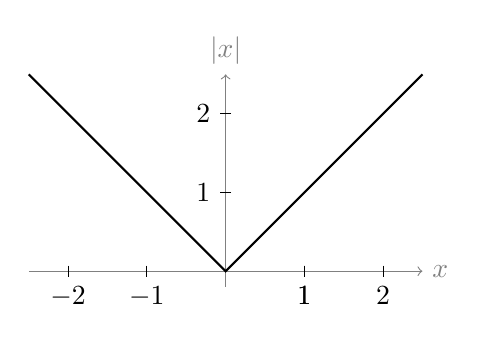
\begin{tikzpicture}[scale=1]
	\draw[->, gray] (-2.5,0) -- (2.5,0) node[right] {$x$};
	\draw[->, gray] (0,-.2) -- (0,2.5) node[above] {$|x|$};
	
	\foreach \x/\xtext in {-2/-2, -1,1, 1/1, 2/2}
	\draw[shift={(\x,0)}] (0pt,2pt) -- (0pt,-2pt) node[below] {{$\xtext$}};
	
	\foreach \y/\ytext in {1/1, 2/2}
	\draw[shift={(0,\y)}] (2pt,0pt) -- (-2pt,0pt) node[left] {{$\ytext$}};
	
	\draw[thick] (-2.5, 2.5)--(0,0)--(2.5, 2.5);
	\end{tikzpicture}
\end{center}
આ વ્યાખ્યા આશરે એમ કહે છે કે~$c$થી
$\delta$ કરતાં ઓછા અંતરે આવેલા
નિવેશો પસંદ કરીને (અર્થાત્ $|x -
c| < \delta$), “ભૂલ”ને
$\epsilon$ કરતાં ઓછી કરી શકાય
(અર્થાત્ $|g(x) - \ell| < \epsilon$).

લક્ષની કલ્પના વ્યાખ્યાયિત કર્યા પછી
અનંતસૂક્ષ્મો વિના જ આગળ વધી શકીએ:
$c$ પર $f$નો ઢાળ આ પ્રમાણે નક્કી કરીએ:
\[
	{f}'(c) = \lim_{x \rightarrow 0}\left(\frac{f(c +x) - f(c)}{x}\right) \text{ જ્યાં લક્ષ અસ્તિત્વમાં હોય}.
\]
પરંતુ વ્યાખ્યામાં “જ્યાં લક્ષ અસ્તિત્વમાં હોય”
એ શરત શા માટે જરૂરી છે તે સમજવું મહત્વનું છે.
હમણાં ચિત્રમાં જોયેલું $f(x) = |x|$
સરળ ઉદાહરણ છે. સ્પષ્ટ છે કે $f'(0)$
સુવ્યાખ્યાયિત નથી: $0$ની “જમણી બાજુથી”
નજીક જઈએ તો ઢાળ હંમેશાં $1$ છે;
$0$ની “ડાબી બાજુથી” જઈએ તો ઢાળ
હંમેશાં $-1$ છે. તેથી લક્ષ અસ્તિત્વમાં
નથી. આથી વિધેય~$f$ બિંદુ~$x$ પર
ત્યારે અને ત્યારે જ \emph{વિકલનીય}
છે જ્યારે આવું લક્ષ અસ્તિત્વમાં હોય.

આપણે જોયું કે \emph{લક્ષ}ની કલ્પનાથી
વિકલનને કેવી રીતે સંભાળી શકાય.
એ જ કલ્પનાથી \emph{સતત} વિધેયનો
ખ્યાલ પણ વ્યાખ્યાયિત કરી શકીએ.
(બોલ્ઝાનોએ 1817 સુધીમાં આ વાતનો
મૂળ વિચાર સમજી લીધો હતો.)
સાતત્ય અંગે કોશી--વાયરસ્ટ્રાસનો
અભિગમ આ પ્રમાણે છે. આશરે કહીએ તો,
વિધેય~$f$ કોઈ બિંદુએ સતત ત્યારે છે
જ્યારે તેના નિર્ગમની ચોકસાઈ અંગેની
કોઈ માંગ તેના નિવેશની ચોકસાઈ
નક્કી કરીને પૂરી કરી શકાય.
વધુ ચોક્કસ રીતે, $f$ બિંદુ $c$
પર સતત છે જો $x$ શૂન્ય તરફ
જાય ત્યારે $f(c + x)$ અને $f(c)$
વચ્ચેનો તફાવત પણ $0$ તરફ જાય.
બીજા શબ્દોમાં, $f$ બિંદુ $c$
પર ત્યારે અને ત્યારે જ
\emph{સતત} છે જ્યારે
$f(c) = \lim_{x \rightarrow c} f(x)$.

આગળ વધીએ તો આપણો વિષય ગણસિદ્ધાંતમાંથી
વાસ્તવિક વિશ્લેષણ તરફ વળી જશે. તેથી
અહીં અટકી આ ચર્ચાનો સાર કહીએ:
ઓગણીસમી સદીમાં ગણિતશાસ્ત્રીઓએ
\emph{લક્ષ}ની ચુસ્ત વ્યાખ્યાયિત કલ્પનાથી
અનંતસૂક્ષ્મો વિના કામ કરવાનું શીખ્યું.
% END OLP-0635
\endgroup

\begingroup
\makeatletter\def\ol@sectioncs{section}\makeatother

% BEGIN OLP-0636
\olfileid{his}{set}{pathology}
\olsection{વિચિત્ર રચનાઓ}
\phantomsection\label{guunit:OLP-0636}


પરંતુ \emph{લક્ષ}ની વ્યાખ્યાએ કેટલીક ખૂબ
“વિચિત્ર” રચનાઓને પણ સ્થાન આપ્યું.

1830ના દાયકાની આસપાસ બોલ્ઝાનોએ એવું
વિધેય શોધ્યું જે \emph{દરેક જગ્યાએ સતત}
પણ \emph{ક્યાંય વિકલનીય નહીં} હતું.
(દુર્ભાગ્યે બોલ્ઝાનોએ આ શોધ પ્રકાશિત
કરી નહોતી; 1872માં વાયરસ્ટ્રાસે સ્વતંત્ર
રીતે એ જ વિચાર શોધ્યો ત્યારે ગણિતશાસ્ત્રીઓને
તે પહેલી વાર જાણ થયો.)\footnote{આ ઇતિહાસ
\href{http://en.wikipedia.org/wiki/Weierstrass_function}{વાયરસ્ટ્રાસ
વિધેય} અંગેના વિકિપીડિયા લેખની અત્યંત
વિગતવાર પાદટીપોમાં નોંધાયેલો છે.}
આ, ઓછામાં ઓછું કહીએ તો, ખૂબ આશ્ચર્યજનક
હતું. $|x|$ જેવું વિધેય શોધવું સહેલું છે
જે દરેક જગ્યાએ સતત હોય પણ કોઈ એક
બિંદુએ વિકલનીય ન હોય. પરંતુ દરેક
જગ્યાએ સતત અને \emph{ક્યાંય}
વિકલનીય ન હોય એવું વિધેય સાવ
જુદી બાબત છે. જરા વિચારો કે
આવું વિધેય કેવી રીતે દોરશો.
સતતતા માટે કાગળ પરથી પેન
ઉઠાવ્યા વિના રેખા દોરી શકાય
એવું હોવું જોઈએ; પરંતુ ક્યાંય
વિકલનીય ન હોય તે માટે પેનની
દિશા સતત એકાએક બદલવી પડે.

પછી આવી બીજી “વિચિત્ર” બાબતો સામે આવી.
5 જાન્યુઆરી 1874ના રોજ કૅન્ટૉરે
ડેડેકિન્ડને પત્ર લખીને આ પ્રશ્ન મૂક્યો:
\begin{quote}
શું કોઈ સપાટીને (દાખલા તરીકે, તેની સીમા
સહિતના ચોરસને) કોઈ રેખા સાથે
(દાખલા તરીકે, અંતબિંદુઓ સહિતની
સીધી રેખા સાથે) એક-એક સંગતતામાં
મૂકી શકાય, જેથી સપાટીના દરેક
બિંદુને રેખાનું એક બિંદુ અને,
ઊલટું, રેખાના દરેક બિંદુને
સપાટીનું એક બિંદુ અનુરૂપ હોય?

હજુ મને આ પ્રશ્નનો ઉત્તર બહુ અઘરો લાગે
છે—જોકે અહીં પણ \emph{ના} કહેવાની
ઇચ્છા એટલી પ્રબળ થાય છે કે તેની
સાબિતી લગભગ અનાવશ્યક ગણવાનું
મન થાય. [\citealt{Gouvea2011}માં
ઉદ્ધૃત]
\end{quote}
પરંતુ 1877માં કૅન્ટૉરે પોતે ખોટા
હોવાની સાબિતી આપી. હકીકતમાં
રેખા અને ચોરસમાં બિંદુઓની
સંખ્યા બરાબર સમાન છે.
29 જૂન 1877ના રોજ તેમણે
ડેડેકિન્ડને લખ્યું:
“\emph{je le vois, mais je ne le crois pas}”;
એટલે, “હું તે જોઈ શકું છું,
પણ તેનો વિશ્વાસ નથી થતો.”
ગણિતના “સ્વીકૃત ઇતિહાસ”માં
આ વાક્ય ઘણી વાર એ દર્શાવતું
માનવામાં આવે છે કે તે સમયના
ગણિતશાસ્ત્રીઓને આ નવાં
પરિણામો \emph{શાબ્દિક અર્થમાં
અવિશ્વસનીય} લાગતાં હતાં.
(પત્રવ્યવહાર \citet{Gouvea2011}માં
આપેલો છે; આપણે
\olref[his][set][mythology]{sec}માં
તેની તરફ ફરી વળીશું.
કૅન્ટૉરની સાબિતીનો
ખાકો \olref[his][set][cantorplane]{sec}માં
આપ્યો છે.)

કૅન્ટૉરના પરિણામથી પ્રેરાઈ પીઆનોએ
વિચાર્યું કે રેખાને સમતલ પર
\emph{સાતત્યપૂર્વક} ચિતરી શકાય કે કેમ.
\sourcecorrection{OLMD-168}{મૂળમાં
\texttt{smoothly} શબ્દ છે. અહીં
ગાણિતિક અર્થમાં વિકલનીય અથવા
મસૃણ ચિત્રણ શક્ય નથી;
પીઆનોનું અવકાશપૂરક ચિત્રણ
સતત છે. તેથી “સાતત્યપૂર્વક”
લખ્યું છે.}
આ \emph{અવકાશ ભરતી વક્રરેખા}
હશે. \citeyear{Peano1890}માં
પીઆનોએ આવી જ વક્રરેખા
રચી. આ ખરેખર સહજ
સમજને પડકારતું છે:
યુક્લિડે રેખાને
“પહોળાઈ વિનાની
લંબાઈ” કહેલી હતી
(પુસ્તક ૧, વ્યાખ્યા ૨),
પરંતુ પીઆનોએ બતાવ્યું
કે રેખાને યોગ્ય રીતે
વાળી તેની લંબાઈથી
પહોળાઈ ભરી શકાય.
\citeyear{Hilbert1891}માં
હિલ્બર્ટે વધુ સહજ
લાગે એવી અવકાશપૂરક
વક્રરેખા અને તેને
દર્શાવતાં ચિત્રો આપ્યાં.
આ વક્રરેખા ક્રમશઃ
રચાય છે; તેના
પ્રથમ છ તબક્કા
અહીં છે:
\begin{center}
\begin{tikzpicture}
\begin{scope}[xshift=20pt, yshift=20pt]
	\draw [oldiagcolorC, l-system={Hilbert curve, step=40pt, angle=90, axiom=L, order=1}] lindenmayer system;
\end{scope}
\begin{scope}[xshift=110pt, yshift=10pt]
	\draw [oldiagcolorC, l-system={Hilbert curve, step=20pt, angle=90, axiom=L, order=2}] lindenmayer system;
\end{scope}
\begin{scope}[xshift=205pt, yshift=5pt]
	\draw [oldiagcolorC, l-system={Hilbert curve, step=10pt, angle=90, axiom=L, order=3}] lindenmayer system;
\end{scope}
\begin{scope}[xshift=2.5pt, yshift=-97.5pt]
	\draw [oldiagcolorC, l-system={Hilbert curve, step=5pt, angle=90, axiom=L, order=4}] lindenmayer system;
\end{scope}
\begin{scope}[xshift=101.25pt, yshift=-98.75pt]
	\draw [oldiagcolorC, l-system={Hilbert curve, step=2.5pt, angle=90, axiom=L, order=5}] lindenmayer system;
\end{scope}
\begin{scope}[xshift=200.625pt, yshift=-99.375pt]
	\draw [oldiagcolorC, l-system={Hilbert curve, step=1.25pt, angle=90, axiom=L, order=6}] lindenmayer system;
\end{scope}
\draw[gray] (0pt,0pt) rectangle (80pt, 80pt);
\draw[gray] (100pt,0pt) rectangle (180pt, 80pt);
\draw[gray] (200pt,0pt) rectangle (280pt, 80pt);
\draw[gray] (0pt,-100pt) rectangle (80pt, -20pt);
\draw[gray] (100pt,-100pt) rectangle (180pt, -20pt);
\draw[gray] (200pt,-100pt) rectangle (280pt, -20pt);
\end{tikzpicture}  
\end{center}
લક્ષ લેતાં—અને હવે લક્ષની ચુસ્ત
વ્યાખ્યા મળી ગઈ છે—આખો
ચોરસ ગાઢ લાલ રંગથી
ભરાઈ જાય છે. વળી,
હિલ્બર્ટની વક્રરેખા
દરેક જગ્યાએ સતત પણ
ક્યાંય વિકલનીય નથી;
સહજ રીતે કહીએ તો,
અનંત લક્ષમાં વિધેય
દરેક ક્ષણે દિશા
એકાએક બદલે છે.
(હિલ્બર્ટની રચનાનો
વધુ વિગતવાર ખાકો
\olref[his][set][hilbertcurve]{sec}માં
આપીશું.)

ભલે સારું કે ખરાબ, આ “વિચિત્ર”
ભૌમિતિક રચનાઓને ભૌમિતિક
સહજજ્ઞાન પર આધાર રાખવા
સામે શંકાનું કારણ માનવામાં
આવી. તે ગણિત કરવાની
નવી રીત માટે લગભગ
\emph{પ્રચાર} બની,
જે આગળ ગણસિદ્ધાંતમાં
પરિણમી. વિષય વિશેની
પછીથી રચાયેલી
દંતકથાઓમાં વારંવાર
કહેવામાં આવતું કે
આ પરિણામો સંપૂર્ણ
ચુસ્ત પણ હતાં અને
સંપૂર્ણ આશ્ચર્યજનક
પણ. તેથી તેમણે
બેવડો હેતુ સાધ્યો:
ભૌમિતિક સહજજ્ઞાન
પર નિર્ભર ન રહેવાની
ચેતવણી આપી અને
નવી વિચારરીતોની
ફળદ્રુપતા બતાવી.
% END OLP-0636
\endgroup

\begingroup
\makeatletter\def\ol@sectioncs{section}\makeatother

% BEGIN OLP-0637
\olfileid{his}{set}{mythology}

\olsection{ઇતિહાસ કરતાં દંતકથા વધુ?}
\phantomsection\label{guunit:OLP-0637}


એક સદીથી વધુ સમય પછી આ ઘટનાઓ તરફ
પાછું જોતાં, આ ચુકાદાઓને તપાસ્યા વિના
સ્વીકારી ન લેવા જોઈએ. પરિણામો ચોક્કસ
નવાં, રોમાંચક અને આશ્ચર્યજનક હતાં.
પરંતુ એ ખરેખર કેટલાં ચોંકાવનારાં હતાં?
અને શું તેમણે ખરેખર બતાવ્યું કે
ભૌમિતિક સહજજ્ઞાન પર આધાર ન રાખવો જોઈએ?

ચોંકાવનારી અસરના પ્રશ્ને,
\citet{Gouvea2011} દર્શાવે છે કે
કૅન્ટૉરે ડેડેકિન્ડને લખેલું પ્રસિદ્ધ
વાક્ય “\emph{je le vois, mais je ne le crois pas}”
ઘણી વાર તેના સંદર્ભથી જુદું કરીને લેવાય છે.
તેનો વધુ સંદર્ભ આ છે
(\citeauthor{Gouvea2011}માંથી ઉદ્ધૃત):
\begin{quote}
વિષય પ્રત્યેના મારા ઉત્સાહને લીધે
હું તમારી દયા અને ધીરજ પાસેથી
આટલી બધી અપેક્ષાઓ રાખું છું,
તે માટે મને માફ કરશો. હાલમાં
તમને મોકલેલી મારી વાતો મને
પોતાને પણ એટલી અણધારી,
એટલી નવી લાગે છે કે, માનનીય
મિત્ર, તેમની સાચાશ વિશે તમારો
નિર્ણય મળે ત્યાં સુધી મને
મનની શાંતિ મળી શકતી નથી.
તમે મારી સાથે સંમત ન થાઓ
ત્યાં સુધી હું એટલું જ કહી
શકું છું: \emph{je le vois, mais je ne le crois pas.}
\end{quote}
કૅન્ટૉર જાણતા હતા કે તેમનું
પરિણામ “એટલું અણધાર્યું,
એટલું નવું” છે. પરંતુ તેમને
પોતાનું પરિણામ ક્યારેય
\emph{અવિશ્વસનીય} લાગ્યું હોય
તે શંકાસ્પદ છે. \citeauthor{Gouvea2011}
દર્શાવે છે તેમ, તેમણે રજૂ કરેલી
સાબિતી ડેડેકિન્ડ તપાસી આપે
એટલું જ તેઓ ઇચ્છતા હતા.

ભૌમિતિક સહજજ્ઞાનના પ્રશ્ને,
પીઆનોએ પોતાની અવકાશ ભરતી
વક્રરેખા કોઈ ચિત્ર વિના
પ્રકાશિત કરી. પરંતુ હિલ્બર્ટે
પોતાની વક્રરેખા પ્રકાશિત
કરી ત્યારે પોતાનો હેતુ સમજાવ્યો:
વાચકો “નીચેના ભૌમિતિક
સહજજ્ઞાનની મદદ લે” તો
પીઆનોનું પરિણામ સમજવાની
સ્પષ્ટ રીત તેમને મળશે.
પછી તેમણે
\olref[his][set][pathology]{sec}માં
આપ્યાં છે તેવાં જ
\emph{ચિત્રો}ની શ્રેણી આપી.

વધુ સામાન્ય રીતે, પ્રકાશિત
સાબિતીઓમાં ચિત્રોનો વપરાશ
થોડો ઓછો થયો હોય, છતાં
ગણિતશાસ્ત્રીઓ સાબિતી કરતી
વખતે ચિત્રોનો \emph{વારંવાર}
ઉપયોગ કરે છે એ હકીકત
ટાળી શકાતી નથી. (સરળ
રીતે કહીએ તો, સારા
ગણિતશાસ્ત્રીઓ જાણે છે કે
ભૌમિતિક સહજજ્ઞાન પર
ક્યારે આધાર રાખી શકાય.)

એટલે આ વાતની અતિશયોક્તિ
માની ન લેવી; ઓછામાં ઓછું,
તપાસ્યા વિના તેનો સ્વીકાર
ન કરવો. વધુ જાણવા
\citet{Giaquinto2007} વાંચી શકો.
% END OLP-0637
\endgroup

\begingroup
\makeatletter\def\ol@sectioncs{section}\makeatother

% BEGIN OLP-0638
\olfileid{his}{set}{cantorplane}
\olsection{રેખા અને સમતલ વિશે કૅન્ટૉર}
\phantomsection\label{guunit:OLP-0638}


શ્રેડર--બર્નસ્ટાઇન પ્રમેયની સાબિતીની
આસપાસની કેટલીક ઘટનાઓ
\olref[his][set][pathology]{sec}માં
ચર્ચેલા ઇતિહાસ સાથે જોડાય છે.
યાદ કરો કે 1877માં કૅન્ટૉરે
ચોરસમાં અને તેની એક બાજુમાં
બિંદુઓની સંખ્યા સરખી છે
તે સાબિત કર્યું હતું. અહીં
તેમની પહેલી પ્રયત્નરૂપ સાબિતી રજૂ કરીએ.

$\unitline$ એકમ રેખા, એટલે
બિંદુઓનો ગણ $[0,1]$,
અને $\unitsquare$ એકમ ચોરસ,
એટલે બિંદુઓનો ગણ $\unitline
\times \unitline$, માનો.
આ સંકેતમાં કૅન્ટૉરે
$\cardeq{\unitline}{\unitsquare}$
સાબિત કર્યું. ડેડેકિન્ડને
લખેલી નોંધમાં તેમણે
મોટા ભાગે નીચેની દલીલ આપી.

\begin{thm}\ollabel{thm:cantorplane}
$\cardeq{\unitline}{\unitsquare}$
\end{thm}

\begin{proof}[સાબિતી: પ્રથમ ભાગ.]
$a, b \in \unitline$ નિશ્ચિત કરો.
તેમને દ્વિઆધારી સંકેતમાં લખો,
જેથી $0$ અને $1$ના અનંત
અનુક્રમો $a_1$, $a_2$, \dots,
અને $b_1$, $b_2$, \dots,
આ રીતે મળે:
\begin{align*}
a &= 0.a_1a_2a_3a_4\dots\\
b &= 0.b_1b_2b_3b_4\dots
\intertext{હવે આ રીતે આપેલું વિધેય $f \colon \unitsquare \to \unitline$ લો:}
f(a, b) & = 0.a_1b_1a_2b_2a_3b_3a_4b_4\dots
\end{align*}
હવે $f$ એ એક-એક વિધેય છે,
કારણ કે જો $f(a, b) = f(c,d)$,
તો દરેક $n \in \Nat$ માટે
$a_n = c_n$ અને $b_n = d_n$;
તેથી $a = c$ અને $b = d$.
\end{proof}

દુર્ભાગ્યે, ડેડેકિન્ડે કૅન્ટૉરને
દર્શાવ્યું તેમ, આ મૂળ પ્રશ્નનો
ઉત્તર આપતું નથી. $0.\dot{1}\dot{0} =
0.1010101010\ldots$ લો.
આને $f(a,b) = 0.\dot{1}\dot{0}$
થવા માટે નીચેના અંકો જોઈએ:
\begin{align*}
a&= 0.\dot{1}\dot{1} = 0.111111\ldots\\
b&= 0
\end{align*}
પરંતુ $a = 0.\dot{1}\dot{1} = 1$ છે.
એટલે “$a$ અને $b$ને દ્વિઆધારી
સંકેતમાં લખો” કહીએ ત્યારે
\emph{કયો} સંકેત લેવો તે પસંદ કરવું
પડે; અને $f$ \emph{વિધેય} હોવું
જોઈએ એટલે બે સંભવિત
સંકેતોમાંથી ફક્ત \emph{એક}
જ લઈ શકીએ. દાખલા તરીકે,
સરળ સંકેત લઈ $a$ને
“$1.000\ldots$” લખીએ,
તો $f(a, b) = 0.\dot{1}\dot{0}$
થાય એવી કોઈ જોડી
$\tuple{a, b}$ મળતી નથી.
\sourcecorrection{OLMD-169}{મૂળનું આ
ઉદાહરણ પસંદ કરેલા સંકેત પર
આધારિત છે: $1$ને
$0.111\ldots$ લખીએ તો
$0.101010\ldots$ ખરેખર
$f(1,0)$ બને છે; અને
$1.000\ldots$ એ ઉપરના
$0.a_1a_2\ldots$ સ્વરૂપમાં નથી.
અવ્યાપ્તતાનું માન્ય ઉદાહરણ
માટે $1$ સિવાયની સંખ્યાઓનું
અંતે માત્ર $1$ આવતું ન હોય
એવું દ્વિઆધારી સ્વરૂપ,
અને $1=0.111\ldots$,
એકસરખી રીતે પસંદ કરો.
પછી $0.00101010\ldots$
સહપ્રદેશમાં છે, પણ તેના
વિષમ સ્થાનોના અંકો
$0.01111\ldots=\frac12$
બને છે; $\frac12$ માટે
પસંદ થયેલું સ્વરૂપ
$0.1000\ldots$ હોવાથી
આ સંખ્યા $f$ની કિંમત
નથી.}

સારાંશમાં, ડેડેકિન્ડે દર્શાવ્યું
કે કેટલાક પુનરાવર્તિત
દ્વિઆધારી વિસ્તરણો શક્ય હોવાથી
કૅન્ટૉરનું વિધેય $f$
એક-એક વિધેય છે, પણ
વ્યાપ્ત વિધેય \emph{નથી}.
તેથી કૅન્ટૉરે ફક્ત
$\cardle{\unitsquare}{\unitline}$
બતાવ્યું છે,
$\cardeq{\unitsquare}{\unitline}$
\emph{નહીં}.

કૅન્ટૉરે લગભગ તરત જ
ડેડેકિન્ડને જવાબ લખીને
સાબિતી નીચે મુજબ
પૂરી કરી શકાય એવું સૂચવ્યું:

\begin{proof}[સાબિતી: પૂર્ણ ભાગ.]
આપણે $\cardle{\unitsquare}{\unitline}$
બતાવ્યું છે. પણ $\unitline$માંથી
$\unitsquare$માં એક-એક વિધેય
સ્પષ્ટ છે: ચોરસની એક બાજુ
પર રેખાને મૂકી દો. તેથી
$\cardle{\unitline}{\unitsquare}$ અને
$\cardle{\unitsquare}{\unitline}$. શ્રેડર--બર્નસ્ટાઇન પ્રમેયથી
(\olref[sfr][siz][sb]{thm:schroder-bernstein}),
$\cardeq{\unitline}{\unitsquare}$.
\end{proof}

અલબત્ત, કૅન્ટૉર આ શબ્દોમાં
છેલ્લી પંક્તિ પૂરી કરી શકતા
નહોતા, કારણ કે શ્રેડર--બર્નસ્ટાઇન
પ્રમેય ત્યારે હજી સાબિત થયું
નહોતું. કૅન્ટૉરે પછી તેને
સામાન્ય અનુમાન તરીકે રજૂ કર્યું,
પરંતુ 1897 સુધી તેની
સંતોષકારક સાબિતી મળી નહોતી.
(એટલે 1877માં જ પછીથી
કૅન્ટૉરે \olref{thm:cantorplane}
માટે શ્રેડર--બર્નસ્ટાઇનનો
આધાર ન લેતી બીજી
સાબિતી આપી.)
% END OLP-0638
\endgroup

\begingroup
\makeatletter\def\ol@sectioncs{section}\makeatother

% BEGIN OLP-0639
\olfileid{his}{set}{hilbertcurve}

\olsection{પરિશિષ્ટ: હિલ્બર્ટની અવકાશ ભરતી વક્રરેખાઓ}
\phantomsection\label{guunit:OLP-0639}


\olref[pathology]{sec} પ્રકરણમાં
આપણે જોયું કે રેખા અને
ચોરસમાં બિંદુઓની સંખ્યા
બરાબર છે એવી કૅન્ટૉરની
સાબિતીએ
(\olref[his][set][cantorplane]{thm:cantorplane})
પીઆનોને પૂછવા પ્રેર્યા કે
શું અવકાશ ભરતી
\emph{વક્રરેખા} હોઈ શકે.
1890માં તેમને તેનો
હકારાત્મક ઉત્તર મળ્યો.
આ વિભાગમાં હિલ્બર્ટની
અવકાશ ભરતી વક્રરેખા
કેવી રીતે રચવી તે
અનૌપચારિક રીતે
સમજાવીએ છીએ
(એક નાનકડા ફેરફાર સાથે).
\footnote{વધુ ચુસ્ત સમજૂતી
માટે \cite{Rose2010} જુઓ.
ફેરફાર એટલે નીચેની
વક્રરેખાઓના લાલ
ભાગો ઉમેરવા; તેથી
વક્રરેખા સતત છે તે
તપાસવું થોડું સહેલું બને છે.}

આપણે વિધેયો $h_1$, $h_2$, $h_3$,
\dots\@ના અનુક્રમના
લક્ષ તરીકે વિધેય $h$
વ્યાખ્યાયિત કરવાનું છે.
પહેલાં રચના વર્ણવીશું,
પછી તે અવકાશ ભરે છે
તે અને અંતે તે
વક્રરેખા છે તે બતાવીશું.

$h$નો વિસ્તાર એકમ ચોરસ
$\unitsquare$ લઈશું.
$h$નો પહેલો અંદાજ,
એટલે $h_1$, આ છે:
\begin{center}
	\begin{tikzpicture}
	\draw[gray] (0pt, 0pt) rectangle (80pt, 80pt);
	\draw[step = 40pt, gray, very thin] (0pt, 0pt) grid (80pt, 80pt);
	\draw[oldiagcolorC, thick] (20pt, 0)--(20pt, 20pt);
	\draw[oldiagcolorC, thick] (60pt, 0)--(60pt, 20pt);		
	\begin{scope}[xshift=20pt, yshift=20pt]
	\draw [black, thick, l-system={Hilbert curve, step=40pt, angle=90, axiom=L, order=1}]  lindenmayer system;
	\end{scope}
	\end{tikzpicture}
\end{center}
રચનાને અનુસરવા ચોરસ પર
$2 \times 2$ની જાળી મૂકી છે.
વક્રરેખા નીચેના ડાબા ચતુર્થાંશથી
શરૂ થઈ ઉપર ડાબે,
પછી ઉપર જમણે અને
અંતે નીચે જમણે જાય
છે એમ વિચારી શકીએ.
રચનાનો બીજો તબક્કો,
એટલે $h_2$, આ છે:
\begin{center}
	\begin{tikzpicture}
	\draw[gray] (0pt, 0pt) rectangle (80pt, 80pt);
	\draw[step = 20pt, gray, very thin] (0pt, 0pt) grid (80pt, 80pt);
	\draw[oldiagcolorC, thick] (0pt, 10pt)--(10pt, 10pt);
	\draw[oldiagcolorC, thick] (70pt, 10pt)--(80pt, 10pt);
	\draw[thick, oldiagcolorE] (10pt, 30pt)--(10pt, 50pt); 
	\draw[thick, oldiagcolorE] (30pt, 50pt)--(50pt, 50pt); 
	\draw[thick, oldiagcolorE] (70pt, 50pt)--(70pt, 30pt); \begin{scope}[xshift=10pt, yshift=30pt]
	\draw [thick, rotate=270,black, l-system={Hilbert curve, step=20pt, angle=90, axiom=L, order=1}]  lindenmayer system;
	\end{scope}
	\begin{scope}[xshift=10pt, yshift=50pt]
	\draw [thick, black, l-system={Hilbert curve, step=20pt, angle=90, axiom=L, order=1}]  lindenmayer system;
	\end{scope}
	\begin{scope}[xshift=50pt, yshift=50pt]
	\draw [thick, black, l-system={Hilbert curve, step=20pt, angle=90, axiom=L, order=1}]  lindenmayer system;
	\end{scope}
	\begin{scope}[xshift=70pt, yshift=10pt]
	\draw [thick, rotate=90,black, l-system={Hilbert curve, step=20pt, angle=90, axiom=L, order=1}]  lindenmayer system;
	\end{scope}
	\end{tikzpicture}
\end{center}
જુદા રંગો $h_2$ની
રચના સમજવામાં મદદ કરશે.
પહેલાં $h_1$ના
લાલ સિવાયના
ભાગની નાની નકલો
ચોરસના નીચે ડાબા,
ઉપર ડાબા, ઉપર જમણા
અને નીચે જમણા
ચતુર્થાંશમાં મૂકીએ
(કાળા રંગમાં).
પછી આ ચાર આકૃતિઓને
લીલી રેખાઓથી
જોડીએ. અંતે આકૃતિને
લાલ રેખાઓથી
ચોરસની સીમા સાથે જોડીએ.

હવે $h_3$ તરફ વળીએ.
$h_1$ના લાલ સિવાયના
ભાગની જોડેલી ચાર નાની
નકલોથી $h_2$ બન્યું,
તે જ રીતે $h_2$ના
લાલ સિવાયના ભાગની
ચાર નાની નકલોથી
$h_3$ બને છે
(કાળા રંગમાં).
પછી તેમને લીલી
રેખાઓથી એકબીજા
સાથે અને અંતે
લાલ રેખાઓથી
ચોરસની સીમા
સાથે જોડીએ.
\begin{center}
	\begin{tikzpicture}
	\draw[gray] (0pt, 0pt) rectangle (80pt, 80pt);
	\draw[step = 10pt, gray, very thin] (0pt, 0pt) grid (80pt, 80pt);
	\draw[thick, oldiagcolorC](5pt, 0pt)--(5pt, 5pt); 
	\draw[thick, oldiagcolorC] (75pt, 0pt)--(75pt, 5pt); 
	\draw[thick, oldiagcolorE] (75pt, 45pt)--(75pt, 35pt);
	\draw[thick, oldiagcolorE] (5pt, 35pt)--(5pt, 45pt); 
	\draw[thick, oldiagcolorE] (35pt, 45pt)--(45pt, 45pt); 
	\draw[thick, oldiagcolorE] (75pt, 45pt)--(75pt, 35pt); \begin{scope}[xshift=5pt, yshift=35pt]
	\draw [rotate=270, thick, black, l-system={Hilbert curve, step=10pt, angle=90, axiom=L, order=2}]  lindenmayer system;
	\end{scope}
	\begin{scope}[xshift=5pt, yshift=45pt]
	\draw [thick, black, l-system={Hilbert curve, step=10pt, angle=90, axiom=L, order=2}]  lindenmayer system;
	\end{scope}
	\begin{scope}[xshift=45pt, yshift=45pt]
	\draw [thick, black, l-system={Hilbert curve, step=10pt, angle=90, axiom=L, order=2}]  lindenmayer system;
	\end{scope}
	\begin{scope}[xshift=75pt, yshift=5pt]
	\draw [thick, rotate=90,black, l-system={Hilbert curve, step=10pt, angle=90, axiom=L, order=2}]  lindenmayer system;
	\end{scope}
	\end{tikzpicture}
\end{center}
આ રીતે $h_n$ પરથી
$h_{n+1}$ વ્યાખ્યાયિત
કરવાની સામાન્ય રીત
દેખાય છે. હવે આ
અનુક્રમી વિધેયો
$h_1$, $h_2$, \dots\@
ના બિંદુવાર લક્ષથી
વક્રરેખા $h$ને
\emph{પોતે} વ્યાખ્યાયિત
કરીએ. એટલે દરેક
$x \in \unitline$ માટે:
\begin{align*}
	h(x) &= \lim_{n \rightarrow \infty} h_n(x)
\end{align*} 
\sourcecorrection{OLMD-170}{મૂળમાં
$x \in \unitsquare$ લખાયું છે,
પણ $h_n$ અને $h$નો
પ્રદેશ $\unitline$ હોવો
જોઈએ. ચિત્રો માત્ર
વક્રરેખાઓના માર્ગ
દર્શાવે છે; દરેક
$h_n$નું પરિમાણીકરણ
અને તેનું બિંદુવાર
લક્ષ અસ્તિત્વમાં છે
તે અહીં સાબિત
થતું નથી.}
હવે આ વક્રરેખા
અવકાશ ભરે છે
તે બતાવીએ.
$h_n$ દોરીએ ત્યારે
$\unitsquare$ પર
$2^n \times 2^n$ની
જાળી મૂકીએ છીએ.
પાયથાગોરસના પ્રમેયથી
જાળીના દરેક કોષના
કર્ણની લંબાઈ છે:
\[
\sqrt{\left(\nicefrac{1}{2^{n}}\right)^2+\left(\nicefrac{1}{2^{n}}\right)^2} = 2^{(\frac{1}{2}-n)}
\]
અને સ્પષ્ટપણે $h_n$
જાળીના દરેક કોષમાંથી
પસાર થાય છે. તેથી
$\unitsquare$નો દરેક
બિંદુ $h_n$ પરના
કોઈ બિંદુથી \emph{વધુમાં વધુ}
$2^{(\frac{1}{2}-n)}$
અંતરે છે. હવે $h$ને
વિધેયો $h_1$, $h_2$,
$h_3$, \dots\@ના લક્ષ
તરીકે વ્યાખ્યાયિત કર્યું છે.
તેથી મૂળની દલીલ પ્રમાણે
કોઈ પણ બિંદુનું $h$થી
મહત્તમ અંતર આ લક્ષ છે:
\[
\lim_{n \rightarrow \infty} 2^{(\frac{1}{2}-n)} = 0.
\]
અર્થાત્, $\unitsquare$નો
દરેક બિંદુ $h$થી
$0$ અંતરે છે. બીજા
શબ્દોમાં, $\unitsquare$નો
દરેક બિંદુ વક્રરેખા
\emph{પર} છે; તેથી
$h$ અવકાશ ભરે છે!{}
\sourcecorrection{OLMD-171}{દરેક
$h_n$ની છબી જાળીના
બધા કોષને મળે છે અને
માત્ર બિંદુવાર લક્ષ
છે, તે પરથી છબી
$h(\unitline)$ આખો
ચોરસ ભરે છે એવો
નિષ્કર્ષ નીકળતો નથી.
તે માટે વિધેયોનું
સમરૂપ અભિસરણ
સ્થાપવું, અને
લક્ષની છબી બંધ છે
તેવું સાતત્ય/સઘનતા
આધારિત પગલું
આપવું પડે.
આ બંને અહીં
અસાબિત છે.}

હવે $h$ ખરેખર
\emph{વક્રરેખા} છે
તે બતાવવાનું બાકી છે.
એ માટે આ ખ્યાલ
વ્યાખ્યાયિત કરવો પડે.
આધુનિક વ્યાખ્યા
જોર્ડને 1887માં
આપેલી વ્યાખ્યા
પર આધારિત છે
(પહેલી અવકાશ ભરતી
વક્રરેખા રજૂ થાય
તેના થોડાં વર્ષ પહેલાં):

\begin{defn}
વક્રરેખા એટલે
$\unitline$માંથી
$\Real^2$માંનું
સતત ચિત્રણ.
\end{defn}

આ વ્યાખ્યા ઘણી સહજ
લાગે છે: સહજ રીતે,
વક્રરેખા પ્રમાણભૂત
રેખાને સમતલ
$\Real^2$ પર લઈ
જતું “મસૃણ” ચિત્રણ
છે. આપણું વિધેય
$h$ ખરેખર
$\unitline$માંથી
$\Real^2$માં જાય છે.
તેથી $h$ સતત
છે તે બતાવવું બાકી છે.
\olref[limits]{sec}માં
આપણે $\epsilon$/$\delta$
સંકેતથી સાતત્ય
વ્યાખ્યાયિત કર્યું હતું.
મૂળની બોલચાલની
વાત આ છે:
\emph{જો તમે $\unitsquare$માં
બિંદુ $p$ અને ઇચ્છિત
ચોકસાઈ $\epsilon$ આપો,
તો $\unitline$નો એવો
ખુલ્લો ભાગ મળે કે
તેમાંના કોઈ પણ $x$
માટે $h(x)$ એ $p$થી
$\epsilon$ કરતાં ઓછા
અંતરે હોય.}
\sourcecorrection{OLMD-172}{અહીં
“મસૃણ” ગણિતીય
વ્યાખ્યા નથી; વ્યાખ્યા
માત્ર સાતત્ય માગે છે.
મૂળનું પછીનું બોલચાલનું
વિધાન પણ સાતત્ય
નથી બતાવતું: તે
દરેક લક્ષ્યબિંદુની
પાસે ક્યાંક આગતોનો
ખુલ્લો ભાગ મળે
એવું કહે છે. સાચી
સાતત્ય-શરત દરેક
$t\in\unitline$
અને $\epsilon>0$
માટે એવો $\delta>0$
માગે છે કે
$|x-t|<\delta$
હોય ત્યારે
$\|h(x)-h(t)\|<\epsilon$
હોય.}

હવે માનો કે તમે
$p$ અને $\epsilon$
આપ્યાં છે. તેનો
અર્થ $\unitsquare$માં
કેન્દ્ર $p$ અને
ત્રિજ્યા $\epsilon$
વાળું વર્તુળ દોરવા
જેવો છે. (વર્તુળનો
ભાગ $\unitsquare$ની
સીમા બહાર જઈ શકે,
પણ તેથી વાંધો નથી.)
યાદ કરો કે $h_n$
વર્ણવતાં આપણે
$\unitsquare$ પર
$2^n \times 2^n$ની
જાળી મૂકી હતી.
$\epsilon$ ગમે તેટલું
નાનું હોય, એવું
કોઈ $n$ મળે છે કે
$\unitsquare$ પરની આ
$2^n \times 2^n$ જાળીના ઓછામાં
ઓછો એક કોષ
કેન્દ્ર $p$ અને
ત્રિજ્યા $\epsilon$
વાળા વર્તુળની
અંદર આખો આવે છે.

એવું $n$ લો અને
$I$ને $\unitline$નો
એવો સૌથી મોટો
ખુલ્લો ભાગ માનો
જેને $h_n$ સંબંધિત
જાળીકોષની અંદર
આખો ચિતરે છે.
($2^n\times 2^n$
જાળીના દરેક કોષમાંથી
$h_n$ પસાર થાય
છે એમ આપણે
નોંધ્યું હોવાથી
એવો $(a,b)$
મળે છે.) હવે
જ્યારે પણ $x \in I$
હોય ત્યારે $h(x)$
એ જ જાળીકોષમાં
રહે છે તે બતાવવું
પૂરતું છે. અને
\emph{આ} માટે
દરેક $m > n$
માટે $h_m(x)$
એ જ કોષમાં
રહે છે તે
બતાવવું પૂરતું છે.
મૂળની દલીલમાં
આ સ્પષ્ટ ગણાય છે:
$m > n$ માટે
$h_m$માં એકમ
અંતરાલનો બરાબર
“એ જ ભાગ”
એ જ જાળીકોષમાં
ચિતરાય છે;
ફક્ત ત્યાં તેની
રચના વધુ લંબાયેલી
અને વળાંકવાળી
થતી જાય છે.
\sourcecorrection{OLMD-173}{આ
દલીલ આપેલા
$p$ની પાસે
વક્રરેખાનો થોડો
ભાગ આવે છે
એવું બતાવવાનો
પ્રયત્ન કરે છે;
પણ દરેક નિશ્ચિત
આગત $t$ની પાસે
$h(x)$ એ $h(t)$ની
પાસે રહે છે,
તે બતાવતી નથી.
વળી “સૌથી મોટો”
ખુલ્લો ભાગ અને
બધાં પછીના
$h_m$ની કોષ-સ્થિરતા
પરિમાણીકરણ
વિના સ્થાપિત
નથી. તેથી અહીં
સાતત્યની સાબિતી
હજી અધૂરી છે.}
% END OLP-0639
\endgroup
% END OLP-0633
\endgroup


\OLEndPartHook
% END OLP-0620
